\chapter{Formally Verified Control-Flow Integrity Micro-Policy}
\label{ch:verified_cfi}

\nick{rephrased the intro, old one in comment. Still needs some iterations.}

In this chapter we develop our main results. In particular, we prove a
property capturing the notion of \CFI, similar to what was proposed by
Abadi \ETAL in \cite{AbadiBEL09}, for the concrete machine running
monitor code that implements the micro-policy of \cref{sec:cfi_fine}.

In order to obtain this result we propose a generic preservation
theorem that states that the \CFI property is preserved, under certain
assumptions, by $\lbrace 0,1 \rbrace$-backward simulation. This
allowed us to structure our proofs in a modular way and to avoid a
direct - and several times more complex - proof of \CFI on the
concrete machine. Furthermore it allowed us to obtain a proof for \CFI
for the Concrete machine by leveraging the micro-policies framework of
\cref{sec:framework} in order to easily obtain a $\lbrace 0,1
\rbrace$-backward simulation between the Concrete and the Symbolic
machine. As a result the proof effort required, was considerably
reduced, as we essentially had to do most of our reasoning at the
Symbolic level.

The reusable nature of our preservation theorem allowed us to use the
Symbolic machine as an intermediate step between an Abstract machine
that has \CFI by construction and therefore a trivial proof of the
\CFI property.  We proved a 1-backward simulation between the Symbolic
and the Abstract machine, which allowed us to invoke the preservation
theorem in order to transfer the \CFI property from the Abstract to
the Symbolic machine and consequently to the Concrete machine by
invoking the preservation theorem for a second time.

Finally, we prove a 1-forward simulation between the Abstract and the
Symbolic machine and thus have a complete two-way refinement between
the Concrete and the Abstract machine. These refinement proofs provide
us with additional assurance in the correctness of our micro-policy.

\nick{mention in the end (here) that our proofs can be found somewhere}

% We proved in Coq that the concrete machine running monitor code that
% implements the micro-policy of \cref{sec:cfi_fine} Using the
% micro-policies framework described in \cref{sec:framework} we proved
% that the concrete machine running monitor code implementing the
% micro-policy in \cref{sec:cfi_fine} \ii{simulates} an abstract machine
% that has \CFI by construction.\ch{Not simulation is the main result;
%   simulation is just a way of proving CFI for the concrete machine,
%   which is the main result and should come first.}  We do this proof
% by using the symbolic machine as an intermediate step, first proving
% backward simulation between the symbolic and the abstract machine and
% afterwards by leveraging the framework of section \cref{sec:framework}
% we obtain a backward refinement between the concrete and the abstract
% machine.

% In addition, we provide an attacker model for all the machines used
% and we prove that a property capturing the notion of \CFI holds even
% when the attacker can tamper all data on the machine, similarly to what is
% proposed in \cite{AbadiBEL09}, but adapted to the setting of our
% machines. We do this by first proving this property for the abstract
% machine and then by using a generic preservation theorem we developed,
% we prove that this property is \emph{preserved} by backward
% refinement and thus transferring the property to the symbolic and
% consequently to the concrete machine. This proof structure, allows us to
% build our proofs in a modular way and additionally reduced the proof
% effort, as it allowed us to reuse the preservation theorem for proving
% \CFI for both the symbolic and the concrete machine and allowed us to
% do most of the reasoning at the symbolic level, even for proofs that
% concerned the concrete machine.

\begin{figure}[H]
  \begin{center}
    \begin{tikzpicture}
      [machine/.style={rectangle,draw=teal!80,text=black,very thick,minimum height=1cm},
       cfi/.style={rectangle,draw,thick,draw=teal!80,text=black,fill=teal!10},
       >=stealth]

      % abstract
      \node [machine,fill=teal!10] (abstract) {Abstract Machine};

      % symbolic-rule
      \node (symbolic label) [below=2.5cm of abstract] {Symbolic Machine};
      \node [rectangle,draw,thick,fill=teal!20,rounded corners]
            (symbolic rules) [right=of symbolic label] {CFI Micro-Policy};
      \begin{pgfonlayer}{background}
        \node [machine,dashed,fill=teal!10,fit={(symbolic label) (symbolic rules)}]
              (symbolic) {};
      \end{pgfonlayer}
      \node [cfi,right=of symbolic] (symbolic cfi) {CFI Property};

      %abstract cfi
      \node [cfi] (abstract cfi)  at (abstract -| symbolic cfi) {CFI Property};
      \draw [thick] (abstract) to (abstract cfi);

      %symbolic cfi
      \draw [thick] (symbolic) to (symbolic cfi);
      \draw [->,thick]
              (abstract cfi)
              to node [right] {Preserved}
              (symbolic cfi);

      % concrete
      \node (concrete label) [below=2.5cm of symbolic label] {Concrete
        Machine};
      \node [rectangle,draw,thick,fill=red!30,rounded corners]
            (fault handler) [right=of concrete label] {CFI Policy Monitor};
      \begin{pgfonlayer}{background}
        \node [machine,dashed,fill=teal!10,fit={(concrete label) (fault handler)}]
              (concrete) {};
      \end{pgfonlayer}
      \node [cfi] (concrete cfi) at (concrete -| symbolic cfi) {CFI Property};
      % \draw [thick,dashed] (concrete) to (concrete cfi);

      \draw [<->,thick]
            (abstract)
            -- node [left] {Simulates}
            (abstract.center |- symbolic.north);

      \draw [<->,thick,dashed]
            (abstract.center |- symbolic.south)
            -- node [left] {Simulates}
            (abstract.center |- concrete.north);

      \draw [thick] (concrete) to (concrete cfi);
      \draw [->,thick]
              (symbolic cfi)
              to[] node [right] {Preserved}
              (concrete cfi);

      % \draw [draw=red!60,thick,->]
      %       (symbolic rules.center |- symbolic rules.south)
      %       -- node [right] {Compiled to}
      %        (symbolic rules.center |- fault handler.north);
    \end{tikzpicture}
  \end{center}
\caption{Diagram explaining proof structure}
\label{proof_structure}
\end{figure}

\Cref{proof_structure} visualizes our proof structure.
Dashes correspond to theorems and definitions provided by
the micro-policies framework, red colored objects correspond
to assumptions we make and the rest to our proofs and definitions.

% \section{Representing control-flow graphs}\label{sec:cfi_tags}

% Our approach for enforcing \CFI, as explained in \cref{sec:cfi_fine},
% requires that we encode the nodes in the control-flow graph in terms
% of identifiers, which in turn are used to tag all sources and targets
% of indirect control-flows.\ch{Give the main idea first, before
%   going into the gory details: we
%   represent a graph as a characteristic function: id to id to bool}

% \ch{I'm starting to wonder whether the level of Coqiness in this
%   subsection is in any way justified. To me it seems like super low
%   level details that nobody will ever care about, and which are not
%   used in any way by the informal statements that follow. So I think
%   that this whole section could be shrunk to the definition of the id
%   to id to bool function, where id a sub-word that's defined somehow
%   in Coq, we don't care, but then it doesn't need to be a section of
%   it's own, but a little note right before you use the cfg the first
%   time. On a similar note, I would remove context annotations with cfi\_id
%   from the other Coq listings.}

% \ch{To express identifiers in Coq ...}%
% At this point we take a detour, to point out an important design point
% of the micro-policies framework and our \CFI micro-policy.  Throughout
% both developments, a heavily parametric and modular approach was
% taken. This parametric design is enabled by the use of the
% \emph{Section} and \emph{Type Classes} mechanisms of Coq. As an
% example, the node identifiers, along with a number of properties we
% require of them are expressed by the following interface (defined in
% terms of a type class):

% \lstheader{id_class}{Interface of node identifiers}
% Context {t : machine_types}.

% Class cfi_id := {
%   id         : eqType;

%   word_to_id : word t -> option id;
%   id_to_word : id -> word t;

%   id_to_wordK : forall x, word_to_id (id_to_word x) = Some x;
%   word_to_idK : forall w x, word_to_id w = Some x -> id_to_word x = w

% }.
% \end{lstlisting}

% The \emph{Context} command on the top of the code above, allows us to
% \textit{assume} that there exists an instance of this interface.
% In fact, the \emph{machine\_types} argument is just another type class,
% serving as a specification of the various types of the machine (\EG the word
% size). This approach allowed us to abstract away from various details and
% structure our proofs in a clean way.
% In addition, we can easily instantiate a different machine with minimal changes
% in our proofs and definitions (\EG instantiate the machine with a different word
% size).

% However, one drawback is that one wrong specification in a type class would
% disallow us to instantiate it and would require that we go back and change
% all parts that used this wrong specification (\EG in our case, the
% \emph{cfi\_id} class was widely used). Therefore one should be careful
% when doing heavy use of such mechanisms.

% Returning to the identifiers, looking at the definition in \cref{id_class},
% we require that the type of the identifiers \id is an Eqtype (has decidable
% boolean equality) and that there exists conversion functions between elements
% of type \word and \id, satisfying some constraints.

% \nick{Should I give some intuition, as to why word\_to\_id is partial? Is it
% obvious?}

% As mentioned in \cref{sec:cfi_fine}, we check for violations of the
% control-flow with respect to a binary relation (on the identifiers)
% \CFG which represents the set of allowed (indirect) jumps. We can
% extend this relation to precisely describe the control-flow of a
% program, by lifting \CFG to a relation \SUCC{} on machine states, that
% includes the set of allowed targets for the rest of the
% instructions. In our Coq development we assumed a translation of
% the allowed jumps in form of a function on two identifiers.


% \lstheader{cfg}{Function on ids representing the set of allowed jumps}
% Variable cfg : id -> id -> bool.
% \end{lstlisting}

% In addition we defined a function valid\_jmp (referred to with the
% notation \J) that expresses the set of allowed jumps between words, by
% using the \emph{word\_to\_id} function.

% \lstheader{valid_jmp}{Function on words representing the set of allowed jumps}
% Definition valid_jmp w1 w2 :=
%   match word_to_id w1, word_to_id w2 with
%     | Some id1, Some id2 => cfg id1 id2
%     | _, _ => false
%   end.
% \end{lstlisting}

\section{Control-Flow Integrity Property}\label{sec:cfi_property}

Our formalization includes a definition of \CFI, similar to the one found in
\cite{AbadiBEL09}, which we prove to be true of all our machines. The need for a
new definition arises from fundamental differences between our enforcement
mechanism on the concrete mechanism and the one used by Abadi \ETAL. In
particular, our enforcement-mechanism does not prevent a violation, instead
it can detect it after it has occurred by taking an arbitrary number of
``protected'' (monitor mode) steps before eventually bringing the machine to a
halt. This does not have any impact on the security effectiveness of our
mechanism, it does however lead to a more complex definition and therefore
more complex proofs.

We draw the identifiers used to tag instructions from a set of
sub-word sized elements, for which there is a partial conversion
function to words ($word\_to\_id$).
We represent the set of allowed indirect jumps, as a characteristic
function on identifiers ($id \rightarrow id \rightarrow bool$), called
\CFG. We can extend this relation to precisely describe the
control-flow of a program, by extending \CFG to a function \SUCC{} on
machine states, that represents the set of allowed targets for all the
instructions. 

The definition of \CFI is further parameterized by an attacker
model. We model the attacker as a step relation
(\stepa{}{}{}). Intuitively the attacker is allowed to change any
\emph{user-level} data but not the code of the program and the \pc, as
well as the tags in the case of a tagged machine.  This limitations
ensures that an attacker cannot directly circumvent the monitor
protection mechanism and our user-level policies (\NWC , \NXD and
\CFI). To account for attacker steps, the stepping relation is
extended as the union of the normal step relation (\stepn{}{}), as
defined by the machine semantics, and the attacker step relation
(\stepa{}{}{}), as defined by the attacker model.

\begin{figure}[htb!]
\centering
\begin{minipage}[b]{0.25\linewidth}
\centering
\infrule[]{\stepn{s}{s'}
  }{\step{s}{s'}}
\label{fig:step_stepn}
\end{minipage}
\hspace{0.5cm}
\begin{minipage}[b]{0.15\linewidth}
\centering
\infrule[]{\stepa{s}{s'}{}
  }{\step{s}{s'}}
\label{fig:step_stepa}
\end{minipage}
\caption{Step relation definition}
\end{figure}

We define a predicate \INITIAL{s}, where s is a machine state, that
states that s is an initial state. We use this predicate to express some
invariants that are preserved through execution (\EG the initial tagging scheme
for the memory). Finally we define a stopping predicate on an execution trace
that states that the machine is coming to a halt with respect to normal steps.

Collecting the above parameters we can define a generic \CFI machine
that we will later instantiate with the Abstract, the Symbolic and the
Concrete machine.

\begin{definition}[CFI Machine]
\label{cfi_machine}
A \CFI machine is a machine parameterized by, a set of states
(\textit{S}), an initial state predicate (\textit{initial}), a step
relation (\stepn{}{}), an attacker step relation (\stepa{}{}{}), a
function that denotes the allowed control-flows for all instructions
(\SUCC{}) and a stopping predicate (\textit{stopping}).
\end{definition}

For a \CFI machine we give the following definitions:

\begin{definition}[Trace has CFI]\label{traceHasCfi}
  We say that an execution trace $s_0 \to s_1 \to \ldots \to s_n$ {\em has CFI}
  if for all $ i \in [0,n)$ if \stepn{s_i}{s_{i+1}} then
  $(s_i,s_{i+1}) \in$ \SUCC{}.
\end{definition}

\nick{The word relation for succ and cfg is strange since they are
booleans, is it ok, or does it confuse you, making you believe they are Props?}

The above definition corresponds to the one found in \cite{AbadiBEL09}, however
it is stronger in the sense that it requires that steps that are in the
intersection of normal and attacker steps respect the control-flow. If we did
not allow for any violations then the above definition would be enough, but
since our enforcement mechanism allows for one violation we have to resort to a
weaker definition.

\begin{definition}[CFI]\label{cfi}
  We say that the machine
  $(\ii{State}, \ii{initial}, \to_n,\allowbreak \to_a, \SUCCm{}, \ii{stopping})$
  has \CFI with respect to the set of allowed indirect jumps \CFG
  if, for any execution starting from initial state $s_0$
  and producing a trace $s_0 \to \ldots \to s_n$, either
  \begin{enumerate}
  \item The whole trace has \CFI according to
    \cref{traceHasCfi}, or else
  \item There is some $i$ such that $s_i \to_n s_{i+1}$,
  and $(s_i, s_{i+1}) \not \in$ \SUCC{}, where
  the sub-traces $s_0 \to \ldots \to s_i$ and
  $s_{i+1} \to \ldots \to s_n$ both have CFI
  and the sub-trace $s_{i+1} \to \ldots \to s_n$ is stopping.
  \end{enumerate}
\end{definition}

\section{The Abstract Machine}\label{sec:abstract_cfi}

The abstract machine has \CFI, \NXD, and \NWC by construction and will
serve as a specification for the symbolic and eventually the concrete
machine that implement \CFI through the tag-based system explained in
the previous chapter.

Unlike the symbolic and the concrete machine, this abstract machine splits the
memory into two disjoint memories, an instruction memory and a data memory. The
instruction memory is fixed (non-writable) and the machine uses this memory to
fetch instructions to execute, so \NWC and \NXD are enforced by construction.

In addition the state of the machine includes an \ok bit, indicating
whether a control-flow violation has occurred or not. The rest of the machine
state is completed by a set of registers and a \pc register. We use a 5-tuple
notation for the state \acfistat{\imem}{\dmem}{\reg}{\pc}{\ok}, where the first
field is the instruction memory, the second the data memory, the third the
registers, the fourth is the pc register and the fifth is the \ok bit.

\subsection{Operational semantics}\label{sec:abstract_semantics}
Below is the step rule for the Store instruction, illustrating both \NWC and
\NXD. Notice that the instruction is fetched by the instruction memory and
the store is done on the data memory.

\begin{figure}[!htb]
\infrule[Store]{
  \imem[\pc] = i \andalso \ii{decode}~i = \ii{Store}~r_p~r_s \andalso
  \rd{\reg}{r_p} = p \\
  \rd{\reg}{r_s} = w \andalso
  \dmem' = \upd{\dmem}{p}{w}
  }{\step{\acfistat{\imem}{\dmem}{\reg}{\pc}{\ii{true}}}{
    \acfistat{\imem}{\dmem'}{\reg'}{\pc+1}{\ii{true}}}}
\caption{Step rule for Store instruction of abstract machine}
\end{figure}

In the above rule, the \ok bit is true for both the starting and the
resulting state. In fact, the machine can take a step only when the
\ok bit is set to true. In the above rule, the \ok bit is set to true
in the resulting state, indicating that no control-flow violation has
happened, as expected by the execution of a Store
instruction. Control-flow violations in the \NWC setting our machine
is executing, can only occur from \emph{indirect} jump instructions,
in our case the Jump and Jal instructions. Upon execution of a Jump or
Jal instruction, we consult the \CFG function to check whether the
change of control-flow is allowed. We do that through a function \J
that converts the words to identifiers and then invokes the \CFG
function on them. If the conversion fails or if it is now allowed
according to \CFG then the jump is taken but the \ok bit is set to
false, which will halt the machine in the next step, as it is only
allowed to step when the \ok bit is set to true. Otherwise the \ok bit
will remain true.

\begin{figure}[!htpb]
\infrule[Jal]{
  \imem[\pc] = i \andalso \ii{decode}~i = \ii{Jal}~r \andalso
  \rd{\reg}{r} = \pc' \\
  \reg' = \upd{\reg}{\ra}{pc+1} \andalso
  \ii{ok} = (\pc,\pc') \in \Jm
  }{\step{\acfistat{\imem}{\dmem}{\reg}{\pc}{\ii{true}}}{
    \acfistat{\imem}{\dmem}{\reg'}{\pc'}{\ii{ok}}}}
\bigskip

\infrule[Jump]{
  \imem[\pc] = i \andalso \ii{decode}~i = \ii{Jump}~r \andalso
  \rd{\reg}{r} = \pc' \andalso
  \ii{ok} = (\pc,\pc') \in \Jm
  }{\step{\acfistat{\imem}{\dmem}{\reg}{\pc}{\ii{true}}}{
    \acfistat{\imem}{\dmem}{\reg'}{\pc'}{\ii{ok}}}}
\caption{Step rules for Jump and Jal instruction of Abstract machine}
\end{figure}

As the abstract machine serves as a specification to a machine with
\CFI, a more intuitive definition of it would not include the \ok bit
and would only allow the Jump and Jal instructions to step if they do
not violate the control-flow graph. However, this abstract machine
would not allow for any violations to occur unlike our enforcement
mechanism for the symbolic and the concrete machine and would lead to
more complex simulation proofs, therefore we do not favor it.

The abstract machine also allows for monitor services to be included,
although the \CFI enforcement mechanism does not require any. We
assume that a monitor service is a privileged action and that it's
execution does not violate the control-flow of the program. Execution
of a monitor service is done simply by jumping to it's address, there
is no separate instruction. As with all other instructions, execution
of the monitor service is only allowed if the \ok bit is set to true.

\begin{figure}[htb!]
\infrule[Service]{
  \pc \not\in \ii{dom(\imem)} \andalso \pc \not\in \ii{dom(\dmem)} \andalso
  \ii{get\_service}~\pc = (addr,f) \\
  f~\acfistat{\imem}{\dmem}{\reg}{\pc}{\ii{true}}=
    \acfistat{\imem}{\dmem'}{\reg'}{\pc'}{\ii{true}}
  }{\stepn{\acfistat{\imem}{\dmem}{\reg}{\pc}{\ii{true}}}{
    \acfistat{\imem}{\dmem'}{\reg'}{\pc'}{\ii{true}}}}
\caption{Step rule for monitor services of abstract machine}
\end{figure}

\TODO{put all rules here in a large figure}

\subsection{Attacker model}\label{sec:abstract_attacker}

The attacker for the abstract machine is allowed to change the
contents of the data memory and the registers \chrev{at any time}
but not the rest of the state.

\begin{figure}[ht]
\infrule{
  \ii{dom}~\dmem = \ii{dom}~\dmem' \andalso
  \ii{dom}~\reg = \ii{dom}~\reg'
}{
  \stepa{\acfistat{\imem}{\dmem}{\reg}{\pc}{\ok}}
  {\acfistat{\imem}{\dmem'}{\reg'}{\pc}{\ok}}
  {A}
}
\caption{Attacker model for the abstract machine}
\end{figure}

\subsection{Allowed control-flows for the abstract machine}
\label{sec:abstract_flow}

We can construct a function \SUCC{A} for the abstract machine
that represents the set of allowed control-flows for all
instructions, by extending the set of allowed jumps \CFG we
introduced earlier.

Below we give a specification of the \SUCC{A} function for the abstract machine,
in the form of inference rules.
A function is defined in the actual Coq development.

\begin{figure}[ht]
\infrule[IndirectFlows]{
  \imem[\pc] = i
  \andalso \ii{decode}~i \in \lbrace \ii{Jal~r}, \ii{Jump~r} \rbrace
  \andalso (\pc,\pc') \in \Jm
  }{
  (\acfistat{\imem}{\dmem}{\reg}{\pc}{\ok} ,
  \acfistat{\imem}{\dmem'}{\reg'}{\pc'}{\ok}) \in \SUCCm{A}}
\bigskip

\infrule[ConditionalFlows]{
  \imem[\pc] = i
  \andalso \ii{decode}~i = \ii{Bnz~r~imm}\\
   (\pc' = \pc + 1) \vee (\pc' = \pc + imm)
  }{
  (\acfistat{\imem}{\dmem}{\reg}{\pc}{\ok} ,
  \acfistat{\imem}{\dmem'}{\reg'}{\pc'}{\ok}) \in \SUCCm{A}}
\bigskip

\infrule[NormalFlows]{
  \imem[\pc] = i
  \andalso
  \ii{decode}~i \not\in \lbrace \ii{Jal~r}, \ii{Jump~r}, \ii{Bnz~r~imm},
  \varnothing \rbrace
  \\ \pc' = \pc + 1
  }{
  (\acfistat{\imem}{\dmem}{\reg}{\pc}{\ok} ,
  \acfistat{\imem}{\dmem'}{\reg'}{\pc'}{\ok}) \in \SUCCm{A}}
\bigskip

\infrule[ServiceFlows]{
  \imem[\pc] = \varnothing \andalso \dmem[\pc] = \varnothing\\
  \ii{get\_service}~\pc = (addr,f)
  }{
  (\acfistat{\imem}{\dmem}{\reg}{\pc}{\ok} ,
  \acfistat{\imem}{\dmem'}{\reg'}{\pc'}{\ok}) \in \SUCCm{A}}
\caption{Allowed control-flows for instructions of the abstract machine}
\end{figure}

Notice that a monitor service is allowed to return anywhere. As we
mentioned before, monitor services at the concrete level, execute in a
protected environment, therefore we do not want to protect their
returns and this is reflected here.

\subsection{Stopping predicate for the Abstract machine}
\label{sec:abstract_stopping}

Finally, we define what it means for the Abstract machine to be ``stopping'' by
defining a predicate on execution traces:

\begin{definition}[Abstract Stopping Predicate]
\label{abstract_stopping}
~
\begin{enumerate}
\item All states in the trace are stuck with respect to normal steps
  (\stepn{}{})
\item All steps in the trace are attacker steps (\stepa{}{}{})
\end{enumerate}
\end{definition}
\ch{Why not give this thing a name/notation? Like this it seems
  like informal handweaving, not a real definition}

\subsection{CFI proof for the Abstract Machine}\label{abstract_proof}

Regarding initial states, we only require that the \ok bit is set to
true.  We can now instantiate the class of the machines defined in
\cref{cfi_machine}, with the abstract machine and prove that the
abstract machine has \CFI according to \cref{cfi}.  We first prove a
helpful lemma, which states a step that is both a normal and an
attacker step is always safe according to the \SUCC{A} function. The
intuition behind this, is that attacker steps retain the \ok bit while
a normal step that violates the control-flow would change the \ok bit
to false.

\begin{lemma}[Step Intersection]
\label{attacker_no_v}
For all states \textit{st, st}' such that \stepa{st}{st'}{A}
and \stepn{st}{st'}, $(\mathit{st},\mathit{st'}) \in \SUCCm{A}$.
\end{lemma}

\begin{proof}
~
\begin{itemize}
\item By the relation \stepn{st}{st'} we know that the \ok bit
of \textit{st} is set to true.
\item The relation \stepa{st}{st'}{A} retains the \ok bit of
\textit{st}, therefore \textit{st'} has the \ok bit set to true.
\item It trivially follows from the definition of \SUCC{A} that
$(\mathit{st},\mathit{st'}) \in \SUCCm{A}$.
\end{itemize}
\end{proof}

\begin{theorem}[Abstract CFI]\label{CFIabstract}
The abstract machine has the \CFI property stated by \cref{cfi}.
\end{theorem}

\begin{proof}
  ~ The proof proceeds by induction on the execution trace.
  \begin{itemize}
  \item \textbf{Base Case} In this case the execution trace is made up
    of a single step \step{st}{st'}. We proceed with case analysis on
    the step.
    \begin{itemize}
    \item \textbf{Attacker Step} By \cref{attacker_no_v} we
      note that an attacker step cannot be a normal step outside the
      \SUCC{A} relation. Thus in this case the whole trace has \CFI
      according to \cref{traceHasCfi}.
    \item \textbf{Normal Step} By case analysis, if
      $(\mathit{st},\mathit{st'}) \in \SUCCm{A}$ then trivially the
      whole trace has \CFI. Otherwise $(\mathit{st},\mathit{st'}) \not
      \in \SUCCm{A}$ and the sub-traces \textit{st} and \textit{st'}
      vacuously have \CFI. In addition the sub-trace \textit{st'} is
      stopping, as the \ok bit of \textit{st'} is set to false and the
      state is stuck with respect to normal steps.
    \end{itemize}
  \item \textbf{Inductive Case} In this case the execution trace is
    extended by an additional step at it's beginning
    $\mathbf{s_0 \to s_1} \to s_2 \to \ldots \to s_n$.
    By the induction hypothesis either:
    \begin{itemize}
    \item The trace $s_1 \to s_2 \to \ldots \to s_n$ has \CFI, by case
      analysis if $(\mathit{s_0},\mathit{s_1}) \in \SUCCm{A}$ the
      whole trace has \CFI. Otherwise $(\mathit{s_0},\mathit{s_1})
      \not \in \SUCCm{A}$, the sub-trace $s_0$ vacuously has \CFI and
      the sub-trace $s_1 \to \ldots \to s_n$ has \CFI by the induction
      hypothesis. Additionally, the sub-trace $s_1 \to \ldots \to s_n$
      is stopping because:
      \begin{itemize}
        \item The whole trace is made up of attacker steps.
           Since $(\mathit{s_0},\mathit{s_1}) \not \in \SUCCm{A}$
           the \ok bit of $s_1$ will be set to false and a normal
           step is not allowed by the operational semantics,
           while attacker steps retain the \ok bit.
         \item The whole trace is stuck with respect to normal steps.
           Trivial from the above.
       \end{itemize}
     \item There exists a step $\stepn{s_{v1}}{s_{v2}}$ such that
       $(\mathit{s_{v1}},\mathit{s_{v2}}) \not \in \SUCCm{A}$ and
       the sub-traces $s_1 \to \ldots \to s_{v1}$ and
       $s_{v2} \to \ldots \to s_n$ both have \CFI and the later
       is also a stopping trace.
       \begin{itemize}
         \item If $(\mathit{s_0},\mathit{s_1}) \in \SUCCm{A}$ then
           \cref{cfi} still holds and the sub-trace $s_1 \to \ldots
           \to s_{v1}$ is extended by one step to $s_0 \to \ldots \to s_{v1}$.
         \item Otherwise the \ok bit for $s_1$ is set to false and the
           rest of the trace is stuck with respect to normal steps. However from
           the induction hypothesis we know that $\stepn{s_{v1}}{s_{v2}}$, which
           is a contradiction.
         \end{itemize}
       \end{itemize}
  \end{itemize}
\end{proof}

\section{The Symbolic  Machine}\label{sec:symbolic_cfi}

The symbolic machine was described in \cref{sec:symbolic}. Unlike the
abstract machine, the symbolic machine has one memory and the
distinction between data and executable instructions is made through
tags, in a fashion similar to what was shown in
\cref{sec:nwc_nxd,sec:cfi_fine}.  We instantiate the symbolic machine,
according to the aforementioned sections, with a set of tags
\TAGS{\DATA,\INSTR{\ii{id}}, \INSTR{\bot}}.

\lstheader{cfi_tags}{Coq definition of Symbolic tags}
Context {ids : @cfi_id t}.

Inductive cfi_tag : Type :=
| INSTR : option id -> cfi_tag
| DATA  : cfi_tag.
\end{lstlisting}

Although enforcement of \CFI does not require any monitor services we
expose the monitor services mechanism and we check whether calls to
each monitor service are allowed or not according to the control-flow
graph. This is done by assuming a lookup-table of monitor services
where each entry has a tag that is used to check for control-flow
violations and a semantic function from symbolic state to symbolic
state which produces the new machine state after execution of the
system call, as shown in \cref{symbolic_step}.

We do not need any internal state for this micro-policy therefore,
only the transfer function is left to implement.

\subsection{Transfer Function}\label{sec:transfer_fun}

We implement the \TRANSFER function based on the rules found in
\ref{sec:cfi_fine}, using Gallina to define a function mapping
input vectors (mvector) to output vectors (rvector).

\lstheader{transfer_coq}{Transfer function for symbolic machine in Coq pseudo-code}
Definition cfi_handler (ivec : Symbolic.IVec cfi_tags) :
           option (Symbolic.OVec cfi_tags (Symbolic.op ivec)) :=
  match ivec with
  | mkIVec   (Jump as op) (Code (Some n))  (Code (Some m))  _
  | mkIVec   (Jal  as op) (Code (Some n))  (Code (Some m))  _  =>
    if cfg n m then
      Some (mkOVec (Code (Some m)) (default_rtag op))
    else
      None
  | mkIVec   (Jump as op)  Data  (Code (Some n))  _
  | mkIVec   (Jal  as op)  Data  (Code (Some n))  _   =>
    Some (mkOVec (Code (Some n)) (default_rtag op))
  | mkIVec   Jump   Data  (Code None)  _
  | mkIVec   Jal    Data  (Code None)  _  =>
    None
  | mkIVec   Store  (Code (Some n))  (Code (Some m))  [_ ; _ ; Data] =>
    if cfg n m then Some (mkOVec Data Data) else None
  | mkIVec   Store  Data  (Code _)  [_ ; _ ; Data]  =>
    Some (mkOVec Data Data)
  | mkIVec   Store  _  _  _  => None
  | mkIVec   op     (Code (Some n))  (Code (Some m))  _  =>
    (* this includes op = Service *)
    if cfg n m then
      Some (mkOVec Data (default_rtag op))
    else
      None
  | mkIVec   op     Data  (Code _)  _  =>
    (* this includes op = Service, fall-throughs checked statically *)
    Some (mkOVec Data (default_rtag op))
  | mkIVec _ _ _ _ => None
  end.
\end{lstlisting}

Although, the rules in \cref{sec:cfi_fine} were fairly simply,
expressing them using Gallina's pattern matching increased their
size. We also experimented, with different ways of writing the
transfer function but we decided to stick with the definition above as
it's the most straightforward. It's worth to note that bugs in the
above definition were easily made apparent when proving theorems
involving the transfer function. In fact, an ``interesting''
experiment was to re-define the above function in a different way and
prove the two equivalent. It took two iterations before getting both
functions to agree and although for small definitions like the one
above, testing or manually reviewing the code will reveal most if not
all bugs, the importance of formal verification in software
engineering and critical software is made obvious even for definitions
that may seem trivial at first. Eventually the correctness of the
transfer function will come from the two-way simulation proofs between
the abstract and the symbolic machine.

\subsection{Attacker model}\label{sec:symbolic_attacker}

Similar to the abstract attacker, the symbolic attacker can change all words
tagged as \DATAname but not the ones tagged as \INSTRname. This is expressed by
the following relations:

\begin{figure}[htbp]
\infrule[AttackData]{
  }{\stepa{\atom{w_1}{\DATA}}{\atom{w_2}{\DATA}}{S}}
\bigskip
\infrule[AttackInstr]{
  }{\stepa{\atom{w_1}{\INSTR{id}}}{\atom{w_1}{\INSTR{id}}}{S}}
\caption{Attacker capabilities}
\label{fig:symbolic_attacker_atom}
\end{figure}

These attacker capabilities on symbolic atoms are lifted to
the memory and registers by a pointwise extension.

\begin{figure}[htbp]
\infrule{
  \stepa{\mem}{\mem'}{S} \andalso
  \stepa{\reg}{\reg'}{S}
}{
  \stepa{\astat{\mem}{\reg}{\atom{\pc}{t_\pc}}{\extra}{}}
  {\astat{\mem'}{\reg'}{\atom{\pc}{t_\pc}}{\extra}{}}
  {S}
}
\caption{Attacker model for the Symbolic machine}
\label{fig:symbolic_attacker}
\end{figure}

\subsection{Allowed control-flows for the Symbolic Machine}
\label{sec:symbolic_flow}

Similar to the abstract machine of \cref{sec:abstract_flow}, we construct
\SUCC{S} for the symbolic machine (\cref{fig:symbolic_succ}) by
extending the set of allowed jumps \CFG.

\begin{figure}[htbp!]
\small
\infrule[IndirectFlows]{
  \mem[\pc] = \atom{\textit{i}}{(\INSTR{src})}
  \andalso \textit{decode~i} \in \lbrace \ii{Jal~r}, \ii{Jump~r} \rbrace\\
  \mem[\pc'] = \atom{\textit{i}'}{(\INSTR{dst})} \\
    (\textit{src},\textit{dst}) \in \CFGm
  }{
  (\acfistat{\mem}{\reg}{\pc}{\extra}{},
  \acfistat{\mem}{\reg}{\pc'}{\extra}{}) \in \SUCCm{S}}
\bigskip

\infrule[IndirectFlows2]{
  \mem[\pc] = \atom{\textit{i}}{(\INSTR{src})}
  \andalso \textit{decode~i} \in \lbrace \ii{Jal~r}, \ii{Jump~r} \rbrace\\
  \mem[\pc'] = \varnothing
    \andalso \textit{get\_service}~\pc = (\INSTR{dst},f) \\
    (\textit{src},\textit{dst}) \in \CFGm
  }{
  (\acfistat{\mem}{\reg}{\pc}{\extra}{},
  \acfistat{\mem}{\reg}{\pc'}{\extra}{}) \in \SUCCm{S}}
\bigskip

\infrule[ConditionalFlows]{
  \mem[\pc] = \atom{\textit{i}}{(\INSTR{_})}
  \andalso \textit{decode~i} = \ii{Bnz~r~imm}\\
   (\pc' = \pc + 1) \vee (\pc' = \pc + imm)
  }{
  (\acfistat{\mem}{\reg}{\pc}{\extra}{},
  \acfistat{\mem}{\reg}{\pc'}{\extra}{}) \in \SUCCm{S}}
\bigskip

\infrule[NormalFlows]{
  \mem[\pc] = \atom{\textit{i}}{(\INSTR{_})}
  \andalso
  \ii{decode}~i \not\in \lbrace \ii{Jal~r}, \ii{Jump~r}, \ii{Bnz~r~imm},
  \varnothing \rbrace
  \\ \pc' = \pc + 1
  }{
  (\acfistat{\mem}{\reg}{\pc}{\extra}{},
  \acfistat{\mem'}{\reg'}{\pc'}{\extra}{}) \in \SUCCm{S}}
\bigskip

\infrule[ServiceFlows]{
  \mem[\pc] = \varnothing \andalso \textit{get\_service}~\pc = (\ti',f)\\
  }{
  (\acfistat{\mem}{\reg}{\pc}{\extra}{},
  \acfistat{\mem'}{\reg'}{\pc'}{\extra'}{}) \in \SUCCm{S}}
\caption{Allowed control-flows for instructions of the symbolic machine}
\label{fig:symbolic_succ}
\end{figure}

\subsection{Initial states of the Symbolic Machine}
\label{sec:symbolic_initial}

For the symbolic machine, we do require that certain tagging
conventions are respected initially. Additionally we prove that
these initial conditions are invariants of the machine and they
are preserved at every (normal or attacker) step.

These invariants are required for backward simulation between
the symbolic and the abstract machine.

\begin{definition}[Instructions Tagged]\label{instructions_tagged}
  ~ For all addresses \textit{addr} in the memory such that
  $$\mem[\mathit{addr}] = \atom{\mathit{i}}{\INSTR{id}}$$ \textit{addr}
  is in the domain of \emph{word\_to\_id} and additionally
  $$word\_to\_id ~\mathit{addr} = \mathit{id}$$
\end{definition}

\begin{definition}[Entry Points Tagged]\label{entry_tagged}
  ~ For all addresses \textit{addr} such that
  \begin{align*}
  & \mem[addr] = \varnothing\\
  & get\_service~addr = (\mathit{it},f)\\
  & \mathit{it} = \INSTR{id}
  \end{align*}
  \textit{addr} is in the domain of \emph{word\_to\_id} and additionally
  $$word\_to\_id ~\mathit{addr} = \mathit{id}$$
\end{definition}

\begin{definition}[Valid Jumps Tagged]\label{valid_jmp_tagged}
  For all addresses \textit{saddr, taddr} such that
  $$(\mathit{saddr},\mathit{taddr}) \in \Jm$$ it holds that
  $$\exists \mathit{i}, \mem[saddr] = \atom{\mathit{i}}{\INSTR{(word\_to\_id~saddr)}} $$
  and either $$\exists \mathit{i'}, \mem[taddr]
  =\atom{\mathit{i'}}{\INSTR{word\_to\_id~taddr}}$$ or
  \begin{align*}
  & \mem[taddr] = \varnothing\\
  & \exists (\mathit{it},f), get\_service~addr = (\mathit{it},f)\\
  & \mathit{it} = \INSTR{(word\_to\_id~taddr)}
  \end{align*}
\end{definition}

Additionally we need two (\TODO{Or three}) more invariants for forward
simulation. These two invariants enforce that all Jump and Jal instructions
are tagged with a unique identifier.

\begin{definition}[Jumps Tagged]\label{jumps_tagged}
  For all addresses \textit{addr} and instructions \textit{i} such
  that $\rd{mem}{addr}=i@\INSTR{x}$ and $decode~i = Jump r$, it holds that
  $$\exists id, word\_to\_id addr = id \land x = id$$
\end{definition}

\begin{definition}[Jals Tagged]\label{jals_tagged}
  For all addresses \textit{addr} and instructions \textit{i} such
  that $\rd{mem}{addr}=i@\INSTR{x}$ and $decode~i = Jal r$, it holds that
  $$\exists id, word\_to\_id addr = id \land x = id$$
\end{definition}

We define a predicate \emph{initial} that determines whether a symbolic
state is an initial state.

\begin{definition}[Symbolic Initial States]\label{symbolic_initial_pred}
  ~ A symbolic state $s^S$ is an initial state ($initial^S ~ s^S$) if
  \cref{instructions_tagged,entry_tagged,valid_jmp_tagged,jumps_tagged,jals_tagged}
  hold for $s^S$ and additionally the tag on the \pc is set to
  \DATAname.
\end{definition}

It's straightforward by the semantics of the step relations to prove
that both normal and attacker steps preserve each of the invariants.
We only need to assume that this holds for monitor services (\IE if we
were to provide some monitor services they would have to preserve
these invariants).

\begin{lemma}[Symbolic Invariants preserved by normal steps]
\label{step_preserves_invariants}
For all symbolic states (\textit{st, st}'),
\begin{align*}
  & \mathit{invariants}~\mathit{st} \implies \\
  & \stepn{\mathit{st}}{\mathit{st}'} \implies \\
  & \mathit{invariants}~\mathit{st}'
\end{align*}
\end{lemma}

\begin{lemma}[Symbolic Invariants preserved by attacker steps]
\label{step_a_preserves_invariants}
For all symbolic states (\textit{st, st}'),
\begin{align*}
  & \mathit{invariants}~\mathit{st} \implies \\
  & \stepa{\mathit{st}}{\mathit{st}'}{S} \implies \\
  & \mathit{invariants}~\mathit{st}'
\end{align*}
\end{lemma}

\subsection{Stopping predicate for the Symbolic Machine}
\label{sec:symbolic_stopping}

Similar to the abstract machine, we say that an execution trace of the
symbolic machine is stopping if:

\begin{definition}[Symbolic Stopping Predicate]
\label{symbolic_stopping}
~
\begin{itemize}
\item All states in the trace are stuck with respect to normal steps
  (\stepn{}{})
\item All steps in the trace are attacker steps (\stepa{}{}{})
\end{itemize}
\end{definition}

\subsection{Symbolic-Abstract  simulation}
\label{sec:refinement_SA}

The Symbolic-Abstract simulation formally defines the connection
between the two machines. We prove a 1-backward simulation theorem for
both normal and attacker steps. This means that every step of the
symbolic machine can be matched by one step of the abstract machine.
Additionally we prove a 1-forward simulation for normal steps,
which means that every step of the abstract machine can be matched
by one on the symbolic machine. Intuitively the above theorems show
that the symbolic machine precisely emulates all behaviors of
the abstract machine.

\begin{definition}[1-Backward Simulation]
\label{simulation_LH}
  A low-level machine simulates a high-level machine with respect to a
  $simulation~relation~\sim$ between low-level machine states and
  high-level machine states, if $s^H_1 \sim s_1^L$ and
  \stepn{s^L_1}{s^L_2} implies that there exists $s^H_2$ such that,
  $s^H_2 \sim s^L_2$ and \stepn{s^H_1}{s^H_2}.

We visualize the above definition with the following diagram:

%
\vspace{-\smallskipamount}
 \begin{center}
    \begin{tikzpicture}
      \matrix (m) [matrix of math nodes,row sep=3em,column sep=4em,minimum width=2em]
      {
        s^L_1 & s^L_2 \\
        s^H_1 & s^H_2 \\};
      \path[->]
      (m-1-1) edge [snake it,-] node  {} (m-2-1)
      edge [above] node [below] {} (m-1-2)
      (m-2-1.east|-m-2-2) edge [dashed] node {}
      node {} (m-2-2)
      (m-1-2) edge [snake it,dashed,-] node {} (m-2-2);
    \end{tikzpicture}
  \end{center}
\vspace{-\smallskipamount}
(Plain lines denote premises, dashed ones conclusions.)
\end{definition}

\begin{definition}[1-Forward Simulation]
\label{fwd_simulation_LH}
  A high-level machine simulates a low-level machine with respect to a
  $simulation~relation~\sim$ between low-level machine states and
  high-level machine states, if $s^H_1 \sim s_1^L$ and
  \stepn{s^H_1}{s^H_2} implies that there exists $s^L_2$ such that,
  $s^H_2 \sim s^L_2$ and \stepn{s^L_1}{s^L_2}.
\end{definition}

Intuitively, backward simulation is enough to capture the desired
security property. Our intuition is further strengthened later, when
we prove that the \CFI property given by \cref{cfi} is preserved by
backward refinement. However, a trivial machine that cannot take any step
also enjoys \CFI vacuously. Forward simulation guarantees that this is not
the case for our symbolic machine and proves that it is a meaningful
implementation of the abstract machine.

\subsubsection{Simulation Relation}
\label{sec:sim_relation}

We define the state simulation relation between the symbolic and
abstract machine by defining the simulation relation for each
component of the state.

\begin{definition}[Data Memory Simulation]\label{refine_dmemory}
  An abstract data memory \dmem is in simulation with a
  symbolic memory \mem, if for all words \textit{w, x} it holds
  that
  $$\rd{\mem}{\mathit{w}} = \atom{x}{\DATA}
  \iff \rd{\dmem}{\mathit{w}} = \mathit{x}$$
\end{definition}

\begin{definition}[Instruction Memory Simulation]
  \label{refine_imemory}
  An abstract instruction memory \imem is in simulation with a
  symbolic memory \mem, if for all words \textit{w, x} it holds
  that
  $$(\exists~\mathit{it}, ~ \rd{\mem}{\mathit{w}} =
  \atom{x}{(\INSTR{\mathit{it}})})
  \iff \rd{\imem}{\mathit{w}} = \mathit{x}$$
\end{definition}

\begin{definition}[Registers Simulation]
  \label{refine_registers}
  An abstract register set \textit{areg} is in simulation with a
  symbolic register set \textit{sreg}, if for all registers \textit{r} and words
  \textit{x} it holds that
  $$ \rd{\mathit{sreg}}{\mathit{r}} = \atom{x}{\DATA})
  \iff \rd{\mathit{areg}}{\mathit{r}} = \mathit{x}$$
\end{definition}

\begin{definition}[PC simulation]
  \label{refine_pc}
  The abstract \pc (\textit{apc}) is in simulation with the symbolic \pc
  ($\atom{\mathit{spc}}{\tpc}$), if it holds that
  $$\mathit{apc} = \mathit{spc} \land
    (\tpc = \DATA \lor \exists\mathit{n \in \id},~
    \tpc = \INSTR{n})$$
\end{definition}

\Cref{refine_dmemory,refine_imemory,refine_registers,refine_pc} relate the basic
components of the state.  What is left to do, is relate the \ok bit of
the abstract machine with the state of the symbolic machine.

\begin{definition}[Correctness]
  \label{refine_correctness}
  The statement of correctness, states that for the symbolic memory
  (\textit{smem}), the symbolic pc ($\atom{spc}{\tpc}$) and the \ok bit
  of the abstract machine, it holds that for all words \textit{i} and
  tags \textit{ti},
  \begin{align*}
     & \rd{\mathit{smem}}{spc} = \atom{i}{ti} \implies \\
     & \ok = true  \iff \\
     & (\forall src \in \id, ~ \tpc = \INSTR{src} \implies  \\
     & ~~\exists dst \in \id, \\
     & ~~~~ \mathit{ti} = \INSTR{dst} \land (src,dst) \in \CFGm)
    \end{align*}
\end{definition}

Informally \cref{refine_correctness} states that if the tag on the
current instruction is \textit{ti}, then if the tag on the pc is set
to \INSTR{src} (which means an indirect flow occurred in the previous
step), there exists an \id dst which is used to tag the current
instruction and additionally the flow from an instruction with \id src
to one with \id dst is allowed according to \CFG, if and only if the
\ok bit of the abstract machine is set to true. This definition
captures the notion that a violation in the abstract machine is also a
violation in the symbolic machine and vice-versa.

We give one more definition of correctness, for the case of monitor
services. The intuition is the same, but because monitor services
live outside the addressable memory of the machines, it's statement
needs to be adapted a bit.

\begin{definition}[Monitor Service Correctness]
  \label{refine_correctness_sc}
  Correctness for monitor services, states that for the symbolic memory
  (\textit{smem}), the symbolic pc ($\atom{spc}{\tpc}$) and the \ok bit
  of the abstract machine, it holds that for all monitor services
  \textit{sc},
  \begin{align*}
     & \rd{\mathit{smem}}{spc} = \varnothing \implies \\
     & \mathit{get\_service}~spc = (\mathit{ti},f) \implies \\
     & \ok = true  \iff \\
     & (\forall src \in \id, ~ \tpc = \INSTR{src} \implies  \\
     & ~~\exists dst \in \id, \\
     & ~~~~ \mathit{ti} = \INSTR{dst} \land (src,dst) \in \CFGm)
    \end{align*}
\end{definition}

The simulation relation ($\sim$) is defined as the conjunction of
\cref{refine_dmemory,refine_imemory,refine_registers,refine_pc,refine_correctness,refine_correctness_sc}
and the invariants
\labelcref{instructions_tagged,entry_tagged,valid_jmp_tagged}.

\subsubsection{Proving 1-backward simulation for normal steps}
\label{sec:backward_SA_normal}

Proving a 1-backward simulation for normal steps is relatively
straight-forward, mostly thanks to the fact that the symbolic
machine abstracts away many details of the concrete machine
that would make the proofs more tedious. Additionally we do
not have to provide such proofs for any monitor service as
we did not use any. Therefore we will only have to reason
about the small set of instructions that the symbolic
and the abstract machine share.

We start with some helpful lemmas about registers and memory
updates. These lemmas serve as the basis for proving simulation for
instructions that change the registers or the memory. The
corresponding Coq definitions and proofs can be found.
\TODO{cite source code/remove this}

\begin{lemma}[Registers Update Backward Simulation]
\label{refine_registers_upd}
For all symbolic register sets (\textit{sreg,sreg}'),
abstract register sets (\textit{areg}), registers (\textit{r}),
words (\textit{v,v}'),
\begin{align*}
  & \mathit{areg} \sim_{regs} \mathit{sreg} \implies \\
  & \rd{\mathit{sreg}}{\mathit{r}} = \atom{v}{\DATA} \implies \\
  & \upd{\mathit{sreg}}{\mathit{r}}{\atom{v'}{\DATA}} = \mathit{sreg'} \implies \\
  & ~~ \exists \mathit{areg'}, \\
  & ~~~~ \upd{\mathit{areg}}{\mathit{r}}{v'} = \mathit{areg'} \land \\
  & ~~~~  \mathit{areg'} \sim_{regs} \mathit{sreg'}
\end{align*}
\end{lemma}

\begin{lemma}[Memory Update Backward Simulation]
\label{refine_memory_upd}
For all symbolic memories (\textit{smem,smem}'),
abstract data memories (\textit{amem}) and
words (\textit{addr,v,v'}),
\begin{align*}
  & \mathit{amem} \sim_{dmem} \mathit{smem} \implies \\
  & \rd{\mathit{smem}}{\mathit{addr}} = \atom{v}{\DATA} \implies \\
  & \upd{\mathit{smem}}{\mathit{addr}}{\atom{v'}{\DATA}} = \mathit{smem'} \implies \\
  & ~~ \exists \mathit{amem'}, \\
  & ~~~~ \upd{\mathit{amem}}{\mathit{addr}}{v'} = \mathit{amem'} \land \\
  & ~~~~  \mathit{amem'} \sim_{dmem} \mathit{smem'}
\end{align*}
\end{lemma}

With these definitions and lemmas we are able to prove 1-backward simulation
for normal steps between the Symbolic and the Abstract machine as defined
by \cref{simulation_LH}, where the low-level machine is the Symbolic machine and
the high-level machine is the Abstract machine.

\begin{theorem}[1-Backward Simulation Symbolic-Abstract]
\label{simulation_SA}
\Cref{simulation_LH} holds for the Symbolic (low-level) and
the Abstract (high-level) machines.
\end{theorem}

\subsubsection{Proving 1-backward simulation for attacker steps}
\label{sec:backward_SA_attacker}

The same definition as \labelcref{simulation_LH} of 1-backward
simulation is used for the attacker, with the sole difference being
that steps now refer to attacker steps.

\begin{definition}[1-Backward Simulation Attacker]
\label{simulation_LH_attacker}
  A low-level machine simulates a high-level machine with respect to
  a $simulation~relation~\sim$ between low-level and high-level machine states,
  if $s^H_1 \sim s^L_1$ and \stepa{s^L_1}{s^L_2}{L} implies that there
  exists $s^H_2$ such that, $s^H_2 \sim s^L_2$ and \stepa{s^H_1}{s^H_2}{H}.
\end{definition}

We prove that 1-backward simulation for attacker steps hold, by first
showing how we can construct attacker steps at the abstract level from
symbolic attacker steps and then showing that this way of building
attacker steps preserves the simulation relation ($\sim$).

A step of the symbolic attacker, as mandated by the semantics of the
attacker model, can only change the memory and register contents tagged
\DATAname, formally \stepa{\mem}{\mem'}{S} and \stepa{\reg}{\reg'}{S}.

Intuitively, we can construct \textit{areg} by \emph{mapping} a function
on the set of registers, that changes a symbolic atom to a word by removing
it's tag.

\lstheader{untag_atom}{Untag symbolic atom function}
Definition untag_atom (a : atom (word t) cfi_tag) := common.val a.
\end{lstlisting}

We can trivially prove that the abstract attacker can take a step
by \emph{mapping} untag\_atom over a symbolic register set. This is
trivial because the attacker can arbitrarily change all registers.

\begin{lemma}[Abstract attacker registers]
\label{areg_map}
  \begin{align*}
    & \stepa{\mathit{sreg}}{\mathit{sreg}'}{S} \implies \\
    & \stepa{\mathit{areg}}{\mathit{map}~untag\_atom~\mathit{sreg}'}{A}
  \end{align*}
\end{lemma}

However, we still need to prove that the simulation relation between
the two machines does not break when attacker steps are taken.
We can proof that simulation of registers is preserved by attacker
steps. The proof proceeds by using the correctness theorem for the map function.
\begin{theorem}[Map Correctness instance]
  $$\rd{(\mathit{map}~\mathit{untag\_atom}~\mathit{sreg}')}{r} =
  \mathit{option\_map}~\mathit{untag\_atom}~ (\rd{\mathit{sreg}'}{r})$$
  where option\_map is defined as
  \lstheader{option_map}{Option Map function}
    Definition option_map f x :=
      match x with
      | Some y => Some (f y)
      | None => None
      end.
  \end{lstlisting}
\end{theorem}

\begin{lemma}[Attacker preserves register simulation]
\label{areg_map_preserves_ref}
  For all abstract register sets (\textit{areg})
  and symbolic register sets (\textit{sreg, sreg}'),
  \begin{align*}
    & \mathit{areg} \sim_{regs} \mathit{reg} \implies \\
    & \stepa{\mathit{sreg}}{\mathit{sreg}'}{S} \implies \\
    & \mathit{map}~untag\_atom~\mathit{sreg}' \sim_{regs} \mathit{sreg}'
  \end{align*}
\end{lemma}

In order to complete the proof of 1-backward simulation for attacker
steps, we also need to construct an abstract memory and to show
that the $\sim_{mem}$ relation is preserved by attacker steps.
Due to the fact that the abstract machine has split data and instruction
memories, in order to follow the same methodology as with registers,
we will need to split the symbolic memory. We achieve this, using a
filter function.

Firstly we proof that attacker steps do not break simulation of
instruction memories. Intuitively this is trivial, as the symbolic
attacker can only change memory contents tagged \DATAname.

\begin{lemma}[Attacker preserves instruction memory simulation]
\label{imem_attacker_ref}
  For all abstract instruction memories (\textit{imem})
  and symbolic memories (\textit{smem, smem'}),
  \begin{align*}
    & \mathit{imem} \sim_{imem} \mathit{smem} \implies \\
    & \stepa{\mathit{smem}}{\mathit{smem}'}{S} \implies \\
    & \mathit{imem} \sim_{imem} \mathit{smem}'
  \end{align*}
\end{lemma}

Constructing a data memory is more complicated than in the previous cases.
Our approach, uses the filter function to create a subset of the symbolic
memory that only contains atoms tagged \DATAname and then applies the
same methodology with registers, mapping the $untag\_atom$ function over
this subset to obtain an abstract data memory.

\lstheader{is_data}{Function that checks if atom is tagged \DATA}
Definition is_data (a : atom (word t) cfi_tag) :=
  match common.tag a with
    | DATA => true
    | INSTR _ => false
  end.
\end{lstlisting}

Again we can prove a few helpful lemmas that ease the final proof.

\begin{lemma}[Attacker preserves data memory simulation]
\label{dmem_attacker_preserves_ref}
  For all abstract data memories (\textit{dmem})
  and symbolic memories (\textit{smem, smem}'),
  \begin{align*}
    & \mathit{dmem} \sim_{dmem} \mathit{smem} \implies \\
    & \stepa{\mathit{smem}}{\mathit{smem}'}{S} \implies \\
    & \mathit{map}~untag\_atom~(\mathit{filter}~\mathit{is\_data}~\mathit{sreg}' \sim_{dmem} \mathit{dmem}'
  \end{align*}
\end{lemma}

The proof of \cref{dmem_attacker_preserves_ref} is slightly more complex than
the one for registers, as we now have to invoke the filter correctness theorem
as well.

\begin{theorem}[Filter Correctness instance]
  $$\rd{(\mathit{filter}~\mathit{is\_data}~\mathit{smem}')}{addr} =
  \mathit{option\_filter}~\mathit{is\_data}~ (\rd{\mathit{smem}'}{addr})$$
  where option\_map is defined as
  \lstheader{option_filter}{Option Filter function}
    Definition option_filter f x :=
      match x with
      | Some x0 => if f x0 then Some x0 else None
      | None => None
      end.
  \end{lstlisting}
\end{theorem}

In all cases, we have to show that the domains of the abstract
memories and registers are also preserved. We include here the
corresponding lemma for the data memory. It's proof was again more
complicated, due to the fact that we had to split the symbolic memory.

\begin{lemma}[Attacker preserves data memory domains]
\label{dmem_attacker_preserves_domain}
  For all abstract data memories (\textit{dmem, dmem}')
  and symbolic memories (\textit{smem, smem}'),
  \begin{align*}
    & \mathit{dmem} \sim_{dmem} \mathit{smem} \implies \\
    & \stepa{\mathit{smem}}{\mathit{smem}'}{S} \implies \\
    & \mathit{dmem}' \sim_{dmem} \mathit{smem}' \implies \\
    & \mathcal{D}(\mathit{dmem}) = \mathcal{D}(\mathit{dmem}')
  \end{align*}
\end{lemma}

Likewise with normal steps, we can now prove a 1-backward
simulation for attacker steps as defined by \cref{simulation_LH_attacker}.

\begin{theorem}[1-Backward Simulation Symbolic-Abstract for Attacker]
\label{simulation_SA_attacker}
\Cref{simulation_LH_attacker} holds for the Symbolic (low-level) and
the Abstract (high-level) machines when the two machines are related
by $\sim$.
\end{theorem}

\subsubsection{Proving 1-forward simulation for normal steps}
\label{sec:forward_SA_normal}

The 1-forward simulation proof between the abstract and the symbolic
machine is similar to the 1-backward simulation proof. Again, we take
the same approach and prove some auxiliary lemmas about memory
and registers updates.

\begin{lemma}[Registers Update Forward Simulation]
\label{refine_registers_upd_fwd}
For all abstract register sets (\textit{areg,areg}'), symbolic
register sets (\textit{sreg}), registers (\textit{r}) and words
(\textit{v'}),
\begin{align*}
  & \mathit{areg} \sim_{regs} \mathit{sreg} \implies \\
  & \upd{\mathit{areg}}{\mathit{r}}{v'} = \mathit{areg'} \implies \\
  & ~~ \exists \mathit{sreg'}, \\
  & ~~~~ \upd{\mathit{sreg}}{\mathit{r}}{\atom{v'}{\DATA}} = \mathit{sreg'} \land \\
  & ~~~~  \mathit{areg'} \sim_{regs} \mathit{sreg'}
\end{align*}
\end{lemma}

\begin{lemma}[Memory Update Forward Simulation]
\label{refine_memory_upd_fwd}
For all abstract data memories (\textit{dmem,dmem}'),
symbolic memories (\textit{smem}) and
words (\textit{addr,v'}),
\begin{align*}
  & \mathit{dmem} \sim_{dmem} \mathit{smem} \implies \\
  & \upd{\mathit{dmem}}{\mathit{addr}}{v'} = \mathit{dmem'} \implies \\
  & ~~ \exists \mathit{smem'}, \\
  & ~~~~ \upd{\mathit{smem}}{\mathit{addr}}{\atom{v'}{\DATA}} = \mathit{smem'} \land \\
  & ~~~~  \mathit{dmem'} \sim_{dmem} \mathit{smem'}
\end{align*}
\end{lemma}

\begin{lemma}[Outside Memory]
\label{refine_memory_none}
For all abstract data memories (\textit{dmem}),
abstract instruction memories (\textit{imem}),
symbolic memories (\textit{smem}) and words (\textit{addr}),
\begin{align*}
  & \mathit{dmem} \sim_{dmem} \mathit{smem} \implies \\
  & \mathit{imem} \sim_{imem} \mathit{smem} \implies \\
  & \rd{\mathit{imem}}{\mathit{addr}} = \varnothing\implies \\
  & \rd{\mathit{dmem}}{\mathit{addr}} = \varnothing\implies \\
  & \rd{\mathit{smem}}{\mathit{addr}} = \varnothing
\end{align*}
\end{lemma}

For proving forward simulation between the abstract and the symbolic
machine it is required that all indirect jumps are tagged with a
unique identifier, which we enforce by the invariants
\labelcref{jumps_tagged,jals_tagged}.

\begin{theorem}[1-Forward Simulation Abstract-Symbolic]
\label{fwd_simulation_SA}
\Cref{fwd_simulation_LH} holds for the Symbolic (low-level) and
the Abstract (high-level) machines.
\end{theorem}

\section{The Concrete  Machine}\label{sec:concrete_cfi}

Assuming the existence of correct code that implements the \CFI
monitor, we can utilize the framework of \cref{sec:framework} to
instantiate the concrete machine and obtain a refinement between the
concrete and the symbolic machines, we need to provide the encoding of
symbolic tags. For the concrete machine we only considered a 32-bit
architecture, but as already mentioned, we could very easily
instantiate the concrete machine with 64-bit words with minimal
changes to our proofs.

\subsection{Concrete tags}\label{sec:concrete_tags}

In order to obtain the concrete tags, we need to wrap the symbolic
tags with the monitor self-protection tags (\USERname, \ENTRYname,
\MONITOR) and provide an encoding to words of these tags.

We use 28 bits for the identifiers. That means, that we can uniquely
identify up to $2^{28}$ instructions. Trying to tag more instructions
than this, would break the symbolic
invariant \labelcref{instructions_tagged}, because by the simulation
relation between the concrete and symbolic machines, the two machines
follow the same tagging scheme for \USERname and \ENTRYname tags.

Defining the conversion functions \footnote{Numbers in the Coq
  definitions are off by one (\EG 27 means 28), for reasons relating
  to the underlying words library} between
words and identifiers is straight forward. We make the
simply choice, to convert words to identifiers only if they
are equal or less than the maximum word our 28-bit identifiers can
fit. Note that this does not mean we reduce the addressable space to
28-bits. You can use addresses higher than $2^{28}$ to place contents
tagged as \DATAname or \MONITOR or even \INSTR{$\bot$} but not
instructions with an identifier.

The conversion from identifiers to words is trivial by
expanding the id to 32-bit words by adding zeros to the high bits.

% \lstheader{id_conversion}{Coq definitions of conversion functions for ids and words}
% Definition id_size := Word.int 27.
% Definition id := [eqType of id_size].
% Definition bound : word t :=
%   Word.repr ((Word.max_unsigned 27) + 1)%Z. (*29 bits*)

% Definition word_to_id (w : word t) : option id_size :=
%   if (Word.ltu w bound) then Some (Word.castu w) else None.

% Definition id_to_word (x : id) : word t :=
%   Word.castu x.
% \end{lstlisting}

% Finally we prove the two properties required by cfi\_id,
% \textit{id\_to\_wordK} and \textit{word\_to\_idK}. We can now
% instantiate cfi\_id with 28-bit sized \textit{ids}.

% \lstheader{cfi_id28}{cfi\_id instance with 28-bit sized \textit{ids}}
% Instance ids : cfi_id := {|
%  id := id;
%  word_to_id := word_to_id;
%  id_to_word := id_to_word
% |}.
% Proof.
%   - by apply id_to_wordK.
%   - by apply word_to_idK.
% Defined.
% \end{lstlisting}

When using identifiers of 28-bits, we can encode the symbolic tags using
30-bits, with an encoding like the one in \cref{tag_encoding}, where
the two least-significant bits are used to distinguish between \DATA,
\INSTR{$\bot$} and \INSTR{\id}, and the 28 higher-bits are the \id
in the last case and zero otherwise.

\begin{table}[float=htb!]
\centering
    \begin{tabular}{|c|c|}
    \hline
    Symbolic Tag   & Encoding \\ \hline
    \DATA           & 0        \\ \hline
    \INSTR{$\bot$}     & 1        \\ \hline
    \INSTR{\id} & $4\id+2$    \\ \hline
    \end{tabular}
  \caption{Encoding of Symbolic Tags}
  \label{tag_encoding}
\end{table}

Having an encoding into 30-bits of symbolic tags, we can use the
2-bits left, to wrap the symbolic tags with the monitor
self-protection tags. We use the two least-significant bits to
distinguish between \USERname (01), \ENTRYname (10) and \MONITOR
(00). Only the \USERname and \ENTRYname wrap around symbolic tags. The
policy monitor does not use symbolic tags and the corresponding tag
\MONITOR does not need to wrap around them. Thus the encoding of the
\MONITOR tag has all its bits set to zero.

\begin{figure}[htb!]
  \centering
  \begin{bytefield}[endianness=big]{32}
    \bitheader{0,1,2,3,31} \\
    \bitbox{28}{id} & \bitbox{1}{1} & \bitbox{1}{0} & \bitbox{1}{0} & \bitbox{1}{1} \\
  \end{bytefield}
  \label{instr_example}
  \caption{Encoding of an instruction with a unique identifier id}
\end{figure}

With the above encoding, we can easily define a \emph{decode} function
and prove that the \emph{decode} function is the \emph{left inverse}
of the \emph{encode} function ($decode (encode~t) = t$) and
\emph{right inverse} for all elements in the domain of \emph{decode}
($decode~w = t \implies encode~t = w$).

\subsection{Concrete-Symbolic backward refinement}\label{sec:refinement_CS}

We can now instantiate the backward refinement between the concrete
and the symbolic machine that is provided by the micro-policies
framework \cite{popl2015}. For the concrete to symbolic backward
refinement we no longer get a 1-backward simulation, due to the fact
that the steps the concrete policy monitor takes are not matched by
any steps of the symbolic machine. For user mode steps (\IE when the
tag of the \pc is \USERname) the framework does provide a proof of
1-backward simulation as defined by \cref{simulation_LH}, with respect
to a simulation relation ($\sim_U$), where the low-level machine is
now the concrete machine and the high-level machine is the symbolic
machine.

For \MONITOR steps a weaker simulation relation ($\sim_M$) is used.
Eventually we obtain a $\lbrace 0,1 \rbrace$-backward simulation between
the concrete and the symbolic machine.

\begin{definition}[Weak simulation relation for Monitor steps]
\label{weak_simulation_relation}
  A concrete state $s^C$ is in weak simulation with a symbolic state $s^S$
  ($s^S \sim_M s^C$), if the tag of the \pc of state $s^C$ is \MONITOR and
  there exists a concrete user state $s_0^C$ such that $s^S \sim_U s^C_0$
  and there is an execution trace $s^C_0 \to_n \ldots \to_n s^C$ formed only by
  monitor steps (all states have \MONITOR tag on the \pc).

  We visualize the above definition with the following diagram:

%
\vspace{-\smallskipamount}
 \begin{center}
    \begin{tikzpicture}
      \matrix (m) [matrix of math nodes,row sep=3em,column sep=4em,minimum width=2em]
      {
        & s^S \\
        s^C_0 & s^C_1 & s^C \\};
      \path[->]
      (m-1-2) edge [snake it,-,above,sloped,font=\tiny] node {U} (m-2-1)
      (m-2-1.east|-m-2-2) edge [below,font=\tiny] node {UM}
      node {} (m-2-2)
      (m-1-2) edge [snake it,-,left,font=\tiny] node {M} (m-2-2)
      (m-2-2.east|-m-2-3) edge [below,font=\tiny] node {$M^*$}
      node {} (m-2-3)
      (m-1-2) edge [snake it,-,above,sloped,font=\tiny] node {M} (m-2-3);
    \end{tikzpicture}
  \end{center}
\vspace{-\smallskipamount}
\end{definition}

We define the simulation relation $\sim_{CS}$ between the concrete
and symbolic machines inductively.

\begin{figure}[htb!]
\centering
\begin{minipage}[b]{0.25\linewidth}
\centering
\infrule[]{s^S \sim_{U} s^C
  }{s^S \sim_{CS} s^C}
\label{cs_user_sim}
\end{minipage}
\hspace{0.5cm}
\begin{minipage}[b]{0.15\linewidth}
\centering
\infrule[]{s^S \sim_{M} s^C
  }{s^S \sim_{CS} s^C}
\label{cs_weak_sim}
\end{minipage}
\caption{Concrete-Symbolic simulation relation}
\end{figure}


\begin{theorem}[$\lbrace 0,1 \rbrace$-Backward simulation between Concrete and Symbolic Machines]
\label{backward_simulation_CS}
  For all concrete states $s^C_1, s^C_2$ and symbolic states $s^S_1$ such that,
  $s^S_1 \sim_{CS} s^C_1$ and \stepn{s^C_1}{s^C_2} it holds that
  $s^S_1 \sim_{CS} s^C_2$ or there exists $s^S_2$ such that
  \stepn{s^S_1}{s^S_2} and $s^S_2 \sim_U s^C_2$.
\end{theorem}

Using the 1-backward simulation between the symbolic and abstract
machines (\cref{simulation_SA}) and the $\lbrace 0,1 \rbrace$-backward
simulation between the concrete and the symbolic machine
(\cref{backward_simulation_CS}), we can obtain our first result, which
is the backward refinement between the concrete machine running a policy
monitor that enforces \CFI and the abstract machine with respect
to a refinement relation ($\sim_{CA}$) between concrete and abstract states.
We define $\sim_{CA}$ in terms of the simulation relation between the
concrete and the symbolic machine ($\sim_{CS}$) and the simulation relation
between the symbolic and the abstract machine ($\sim_{SA}$).

\begin{figure}[htb!]
\infrule[]{
  s^S \sim_{CS} s^C \andalso s^A \sim_{SA} s^S
  }{s^A \sim_{CA} s^C}
\caption{Refinement relation between Concrete and Abstract machines}
\label{refinement_CA}
\end{figure}

\begin{theorem}[Concrete-Abstract backward refinement]
\label{backward_refinement_CA}
  For all abstract machine states ($s^A_1$), concrete machine states
  ($s^C_1, s^C_2$), if $s^A_1 \sim_{CA} s^C_1$ and
  $s^C_1 \to_n^{*} s^C_2$ and $s^C_2$ is in user mode, then
  there exists an abstract machine state $s^A_2$ such that
  $s^A_1 \to_n^{*} s^A_2$ and $s^A_2 \sim_{CA} s^C_2$.
\end{theorem}

In order to obtain our second result, which is a proof that the
property stated by \cref{cfi} holds for the concrete machine, we will
need to make the concrete machine an instance of
the \labelcref{cfi_machine}, by defining all it's parameters, similar
to what we did for the abstract and symbolic machines.

\subsection{Attacker model}\label{sec:concrete_attacker}

The attacker model for the concrete machine, models an attacker that
can tamper with the machine only when it's in user mode. The
capabilities of the concrete attacker when the machine is in user
mode, directly matches the capabilities of the symbolic attacker,
which means that the attacker can only change the values of atoms that
have a \USERname tag. This prevents the attacker from changing monitor
data in memory or registers, as well as the tags.

\begin{figure}[htb!]
\infrule[AttackUser]{
  \stepa{\atom{w_1}{ut_1}}{\atom{w_2}{ut_2}}{S}
  }{\stepa{\atom{w_1}{\USER{ut_1}}}{\atom{w_2}{\USER{ut_2}}}{C}}
\caption{Concrete attacker capabilities on atoms}
\label{concrete_attacker_atom}
\end{figure}

\begin{figure}[htb!]
\infrule{
  \stepa{\mem}{\mem'}{C} \andalso
  \stepa{\reg}{\reg'}{C}
}{
  \stepa{\cstat{\mem}{\reg}{\cache}{\atom{\pc}{\USER{ut}}}{\epc}}
  {\cstat{\mem'}{\reg'}{\cache}{\atom{\pc}{\USER{ut}}}{\epc}}
  {C}
}
\caption{Attacker model for the Concrete machine}
\label{concrete_attacker}
\end{figure}

\subsection{Concrete-Symbolic 1-backward simulation for Attacker}
\label{sec:backward_CS_attacker}

For attacker steps we can prove a 1-backward simulation, instantiating
\cref{simulation_LH}, with the concrete machine as the low level machine,
the symbolic machine as the high machine and using $\sim_U$ as a simulation
relation.

In order to prove the simulation, we apply the same technique as in the
case of Symbolic-Abstract backward simulation for attacker steps, constructing
attacker steps at the symbolic level from attacker steps in the concrete level
and additionally showing that the way we build the steps preserve the simulation
relation.

We can construct a symbolic memory and a symbolic set of registers
from their concrete counterparts by filtering all non-user data of the
concrete memory and registers and then decoding all the concrete tags
to symbolic ones. We can achieve this using the filter and map
functions as seen in \cref{sec:backward_SA_attacker}.

\lstheader{is_user}{Function that returns true if atom has a \USERname tag}
Definition is_user (x : atom (word mt) (word mt)) :=
  rules.word_lift (fun t => rules.is_user t) (common.tag x).
\end{lstlisting}

\lstheader{coerce}{Function that converts a concrete atom to a symbolic one}
Definition coerce (x : atom (word mt) (word mt))
   : atom (word mt) (cfi_tag) :=
   match rules.decode (common.tag x) with
   | Some (rules.USER tg) => (common.val x)@tg
   | _ => (common.val x)@DATA (*this is unreachable in our case*)
   end.
\end{lstlisting}

We can now prove \cref{creg_simulation,cmem_simulation} the two lemmas that
will allows us to easily proof the 1-backward simulation for attacker steps.

\begin{lemma}[Concrete-Symbolic attacker registers 1-backward simulation]
\label{creg_simulation}
  For all symbolic register sets (\textit{sreg})
  and concrete register sets (\textit{creg, creg}'),
  \begin{align*}
    & \mathit{sreg} \sim_{regs} \mathit{creg} \implies \\
    & \stepa{\mathit{creg}}{\mathit{creg}'}{C} \implies \\
    & \stepa{sreg}{\mathit{map}~coerce~(filter~is\_user~\mathit{creg}')}{S}
  \end{align*}
\end{lemma}

\begin{lemma}[Concrete-Symbolic attacker memory 1-backward simulation]
\label{cmem_simulation}
  For all symbolic memories (\textit{smem})
  and concrete memories (\textit{cmem, cmem}'),
  \begin{align*}
    & \mathit{smem} \sim_{mem} \mathit{cmem} \implies \\
    & \stepa{\mathit{cmem}}{\mathit{cmem}'}{C} \implies \\
    & \mathit{map}~coerce~(filter~is\_user~\mathit{cmem}') \sim_{mem}
       \mathit{cmem}' \\
    & \stepa{smem}{\mathit{map}~coerce~(filter~is\_user~\mathit{cmem}')}{S}
  \end{align*}
\end{lemma}

We additionally have to prove that attacker steps preserve some low-level
invariants of the concrete machine that are required by the framework we
use, but the proofs are mostly trivial as the invariants regard pieces of
state the attacker cannot tamper with \EG monitor data.

\begin{theorem}[1-Backward Simulation Concrete-Symbolic for Attacker]
\label{simulation_CS_attacker}
\Cref{simulation_LH_attacker} holds for the Concrete (low-level) and
the Symbolic (high-level) machines when the two machines are related
by $\sim_U$.
\end{theorem}

\subsection{Allowed control-flows for the Concrete Machine}
\label{sec:concrete_flow}

Once again we construct a function that decides the validity of all
control-flows \SUCC{C}, this time for the concrete machine. \SUCC{C}
allows all flows involving monitor mode and only restricts
the control-flow for user mode execution.

\begin{figure}[htb!]
\small
\infrule[MonitorFlows]{
   in\_monitor~s_1~||~in\_monitor~s_2
  }{(s_1, s_2) \in \SUCCm{C}}
\bigskip

\infrule[IndirectFlows]{
  \mem[\pc] = \atom{\textit{i}}{\USER{(\INSTR{src})}}
  \andalso \textit{decode~i} \in \lbrace \ii{Jal~r}, \ii{Jump~r} \rbrace\\
  \mem[\pc'] = \atom{\textit{i}'}{\USER{(\INSTR{dst})}} \\
  \tpc = \USER{\textit{ut}}
  \andalso \tpc' = \USER{\textit{ut}'}
  \andalso (\textit{src},\textit{dst}) \in \CFGm
  }{
  (\cstat{\mem}{\reg}{\cache}{\atom{\pc}{\tpc}}{\epc},
  \cstat{\mem}{\reg}{\cache}{\atom{\pc'}{\tpc'}}{\epc}) \in \SUCCm{C}}
\bigskip

\infrule[IndirectFlows2]{
  \mem[\pc] = \atom{\textit{i}}{\USER{(\INSTR{src})}}
  \andalso \textit{decode~i} \in \lbrace \ii{Jal~r}, \ii{Jump~r} \rbrace\\
  \mem[\pc'] = \atom{\textit{i}'}{\ENTRY{(\INSTR{dst})}} \\
  \tpc = \USER{\textit{ut}}
  \andalso \tpc' = \USER{\textit{ut}'} \\
  \textit{decode~i}' = \textit{Nop} \andalso (\textit{src},\textit{dst}) \in \CFGm
  }{
  (\cstat{\mem}{\reg}{\cache}{\atom{\pc}{\tpc}}{\epc},
  \cstat{\mem}{\reg}{\cache}{\atom{\pc'}{\tpc'}}{\epc}) \in \SUCCm{C}}
\bigskip

\infrule[ConditionalFlows]{
  \mem[\pc] = \atom{\textit{i}}{\USER{(\INSTR{\_})}}
  \andalso \textit{decode~i} = \ii{Bnz~r~imm} \\
  \tpc = \USER{\textit{ut}}
  \andalso \tpc' = \USER{\textit{ut}'} \\
  (\pc' = \pc + 1) \vee (\pc' = \pc + imm)
  }{
  (\cstat{\mem}{\reg}{\cache}{\atom{\pc}{\tpc}}{\epc},
  \cstat{\mem}{\reg}{\cache}{\atom{\pc'}{\tpc'}}{\epc}) \in \SUCCm{C}}
\bigskip

\infrule[NormalFlows]{
  \mem[\pc] = \atom{\textit{i}}{\USER{(\INSTR{\_})}}
  \andalso
  \ii{decode}~i \not\in \lbrace \ii{Jal~r}, \ii{Jump~r}, \ii{Bnz~r~imm},
  \varnothing \rbrace\\
  \tpc = \USER{\textit{ut}}
  \andalso \tpc' = \USER{\textit{ut}'} \\
  (\pc' = \pc + 1) \vee (\pc' = \pc + imm)
  }{
  (\cstat{\mem}{\reg}{\cache}{\atom{\pc}{\tpc}}{\epc},
  \cstat{\mem'}{\reg'}{\cache}{\atom{\pc'}{\tpc'}}{\epc}) \in \SUCCm{C}}

\caption{Allowed control-flows for instructions of the concrete machine}
\label{concrete_succ}
\end{figure}

\subsection{Initial states of the Concrete Machine}
\label{sec:concrete_initial}

For the concrete machine, we require that it's initial states matches
the initial states of the symbolic machine under the simulation
relation $\sim_U$. This ensures that concrete initial states satisfy
both the invariants we enforced on symbolic initial states and any
low-level invariants enforced by $\sim_U$.

\begin{definition}[Concrete Initial States]\label{concrete_initia_pred}
  ~ A concrete state $s^C$ is an initial state if there exists a
  symbolic state $s^S$ such that $initial^S ~ s^S$ and $s^S \sim_U
  s^C$.
\end{definition}

\subsection{Stopping predicate for the Concrete Machine}
\label{sec:concrete_stopping}

The stopping predicate for the concrete machine is more complex than
the one for the symbolic or the abstract machine, due to the monitor
steps. In particular, on the next step after a violation the machine
will enter monitor mode to determine whether the step is allowed or
not. The miss handler will take an arbitrary number of steps to
determine that execution should be disallowed because a violation of
the policy occurred. This is modeled by disallowing the concrete
machine to return to user mode.  However, note that it could be the
case that the machine cannot step at all after a control-flow
violation, for example if the \pc is outside the memory of the machine.

In addition to the above, there may be attacker steps. These can only
come immediately after the violating step and before the machine
enters monitor mode. Attacker is not allowed to take steps during
monitor mode and as mentioned above the machine will not return to
user mode.

We can summarize the conditions that hold for an execution trace to
be stopping.

\begin{definition}[Concrete Stopping Predicate]
\label{concrete_stopping}
~
\begin{itemize}
\item There is an optional prefix of attacker steps (\stepa{}{}{C}) and
  all states in the prefix are user states.
\item There is an optional suffix of monitor steps (\stepn{}{}) and
  all states in the suffix are monitor steps.
\end{itemize}

\begin{center}
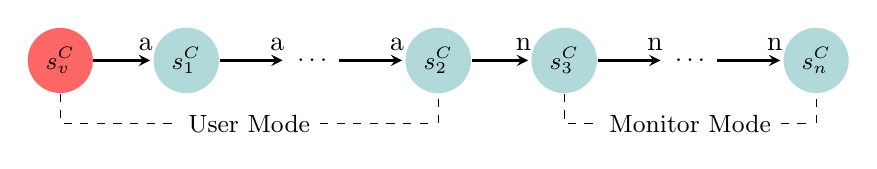
\begin{tikzpicture}
  [scale=.8,auto=left,shorten >=1pt,every node/.style={circle,fill=teal!30,font=\small},->,>=stealth]
  \node (nv) [style={fill=red!60}] at (0,0)  {$s^C_v$};
  \node (na1) at (2,0)  {$s^C_1$};
  \node (nadots) [draw=none,style={fill=white}] at (4,0)  {$\ldots$};
  \node (na2) at (6,0)  {$s^C_2$};
  \node (nm1) at (8,0)  {$s^C_3$};
  \node (nmdots) [draw=none,style={fill=white}] at (10,0)  {$\ldots$};
  \node (nm2) at (12,0)  {$s^C_n$};

\node (nulabel) [rectangle,fill=white,font=\small] at (3,-1) {User Mode};
\node (na2label) [fill=none] at (6,-1) {};

\node (nmlabel) [rectangle,fill=white,font=\small] at (10,-1) {Monitor Mode};
\node (nm2label) [fill=none] at (12,-1) {};

\draw[-,dashed,very thin] (nv) |- (nulabel);
\draw[-,dashed,very thin] (nulabel.east) |- (na2label.center);
\draw[-,dashed,very thin] (na2label.center) |- (na2.south);

\draw[-,dashed,very thin] (nm1) |- (nmlabel);
\draw[-,dashed,very thin] (nmlabel.east) |- (nm2label.center);
\draw[-,dashed,very thin] (nm2label.center) |- (nm2.south);

\path[thick, every node/.style={}]
(nv) edge [very near end,above] node {a} (na1)
(na1) edge [very near end,above] node {a} (nadots)
(nadots) edge [very near end,above] node {a} (na2)
(na2) edge [very near end,above] node {n} (nm1)
(nm1) edge [very near end,above] node {n} (nmdots)
(nmdots) edge [very near end,above] node {n} (nm2);
\end{tikzpicture} \\
\end{center}
\end{definition}

\section{Generic Preservation Theorem}
\label{sec:cfi_preservation}

In this section, we discuss the preservation theorem that we used,
along with the simulation proofs of
\cref{sec:refinement_SA,sec:refinement_CS}, in order to prove \CFI
(\cref{cfi}) for the concrete machine.

The statement of the theorem is parameterized by two \CFI machines
(\cref{cfi_machine}. Moreover, we require that a $\lbrace 0,1
\rbrace$-backward simulation between the two machines, holds for
normal steps and a 1-backward simulation for attacker steps.  The
$\lbrace 0,1 \rbrace$ simulation for normal steps, stems from the fact
that the steps of the concrete machine in monitor mode are not matched
by any steps on the symbolic (or the abstract) level. We generalize
this, by a notion of \emph{checked steps} on the steps of the
low-level machine. Intuitively we only check for control-flow
violations when a checked step is taken.

We require a strong 1-backward simulation for checked steps and
a $\lbrace 0,1 \rbrace$-backward simulation for the rest.

\begin{minipage}{\linewidth}
  \centering
  \begin{minipage}{0.45\linewidth}
    \begin{figure}[H]
      \begin{center}
        \begin{tikzpicture}
          \matrix (m) [matrix of math nodes,row sep=3em,column sep=4em,minimum width=2em]
          {
            s^L_1 & s^L_2 \\
        s^H_1 & s^H_2 \\};
      \path[->]
      (m-1-1) edge [snake it,-] node {} (m-2-1)
      edge [above] node [above,very near end,font=\small] {n} (m-1-2)
      (m-2-1.east|-m-2-2) edge [dashed, above,very near end,font=\small] node {n}
      node {} (m-2-2)
      (m-1-2) edge [snake it,dashed,-] node {} (m-2-2);
    \end{tikzpicture}
       \end{center}
       \caption{1-backward simulation}
     \end{figure}
  \end{minipage}
  \hspace{0.05\linewidth}
  \begin{minipage}{0.45\linewidth}
    \begin{figure}[H]
      \begin{center}
        \begin{tikzpicture}
          \matrix (m) [matrix of math nodes,row sep=3em,column sep=4em,minimum width=2em]
          {
            s^L_0 & s^L_1 \\
            s^H\\};
          \path[->]
          (m-1-1) edge [snake it,-,above] node {} (m-2-1)
          (m-1-1.east|-m-1-2) edge [above,font=\small, very near end] node {n}
          node {} (m-1-2)
          (m-1-2) edge [snake it,dashed,-] node {} (m-2-1);
        \end{tikzpicture}
      \end{center}
      \caption{0-backward simulation}
    \end{figure}
  \end{minipage}
\hspace{0.05\linewidth}
  \begin{minipage}{0.45\linewidth}
    \begin{figure}[H]
      \begin{center}
        \begin{tikzpicture}
          \matrix (m) [matrix of math nodes,row sep=3em,column sep=4em,minimum width=2em]
          {
            s^L_1 & s^L_2 \\
            s^H_1 & s^H_2 \\};
          \path[->]
          (m-1-1) edge [snake it,-] node {} (m-2-1)
          edge [above] node [above,very near end,font=\small] {a} (m-1-2)
          (m-2-1.east|-m-2-2) edge [dashed, above,very near end,font=\small] node {a}
          node {} (m-2-2)
          (m-1-2) edge [snake it,dashed,-] node {} (m-2-2);
        \end{tikzpicture}
      \end{center}
      \caption{1-backward simulation for attacker}
    \end{figure}
    \bigskip
  \end{minipage}
\end{minipage}

Formally we capture the above specifications with the following definitions:

\begin{definition}[$\lbrace 0,1\rbrace$-Backward Simulation for normal steps]
\label{backward_simulation_preservation}
  For all states $s^H_1$ of the high-level machine and $s^L_1, s^L_2$ of
  the low-level machine, such that $s^H_1 \sim s^L_1$ and $s^L_1 \to_n s^L_2$
  with a checked step, there exists $s^H_2$ such that,
  $s^H_2 \sim s^L_2$ and \stepn{s^H_1}{s^H_2}.
  If $s^L_1 \to_n s^L_2$ is an unchecked step then either the same as above
  holds or $s^H_1 \sim s^L_2$.
\end{definition}

\begin{definition}[1-Backward Simulation for attacker steps]
\label{backward_simulation_a_preservation}
  \Cref{simulation_LH} holds for attacker steps.
\end{definition}

% \lstheader{machine_refinement}{Interface of machine\_refinement\ch{
%   Wouldn't this look better in LaTeX than in Coq?}}
% Variable amachine : cfi_machine. (*high-level machine*)
% Variable cmachine : cfi_machine. (*low-level machine*)

% (* General notion of refinement between two machines*)
% Class machine_refinement
%   (amachine : cfi_machine) (cmachine : cfi_machine) := {
%     refine_state : (@state amachine) -> (@state cmachine) -> Prop;

%     check : (@state cmachine) -> (@state cmachine) -> bool;

%     backward_refinement_normal :
%       forall ast cst cst'
%         (REF: refine_state ast cst)
%         (STEP: step cst cst'),
%         (check cst cst' = true ->
%         exists ast', step ast ast' /\ refine_state ast' cst')
%         /\ (check cst cst' = false ->
%              refine_state ast cst' \/
%              exists ast', step ast ast' /\ refine_state ast' cst');

%     backward_refinement_attacker :
%       forall ast cst cst'
%         (REF: refine_state ast cst)
%         (STEPA: step_a cst cst'),
%         exists ast', step_a ast ast' /\ refine_state ast' cst'
% }.
% \end{lstlisting}

From these relations on single steps, we can build a refinement
relation on execution traces. We define this trace refinement relation
inductively and we say that two traces are in refinement if they
are built this way.

\begin{figure}[ht]
\infrule[TRNil]{
  s^H \sim s^L
  }{ s^H \simtr{} s^L }
\bigskip

\infrule[TRNormal0]{
  \stepn{s^L_1}{s^L_2} \andalso \neg check~s^L_1~s^L_2 \\[0.4em]
  s^H_1 \sim s^L_1 \andalso s^H_2 \sim s^L_2 \\[0.4em]
  s^H_1 \cdot tr^H \simtr{} s^L_2 \cdot tr^L
  }{
    s^H_1 \cdot tr^H \simtr{} s^L_1 \cdot s^L_2 \cdot tr^L}
\bigskip

\infrule[TRNormal1]{
  \stepn{s^L_1}{s^L_2} \andalso \stepn{s^H_1}{s^H_2} \\[0.4em]
   s^H_1 \sim s^L_1 \andalso s^H_2 \sim s^L_2 \\[0.4em]
   s^H_2 \cdot tr^H \simtr{} s^L_2 \cdot tr^L
  }{
    s^H_1 \cdot s^H_2 \cdot tr^H \simtr{} s^L_1 \cdot s^L_2 \cdot tr^L}
\bigskip

\infrule[TRAttacker]{
  \stepa{s^L_1}{s^L_2}{} \andalso \stepa{s^H_1}{s^H_2}{} \andalso s^L_1 \not \to_n s^L_2\\[0.4em]
   s^H_1 \sim s^L_1 \andalso s^H_2 \sim s^L_2 \\[0.4em]
   s^H_2 \cdot tr^H \simtr{} s^L_2 \cdot  tr^L
  }{
    s^H_1 \cdot s^H_2 \cdot tr^H \simtr{} s^L_1 \cdot s^L_2 \cdot tr^L}
\caption{Trace refinement relation}
\label{refine_traces}
\end{figure}


In \cref{refine_traces} we distinguish between three separate cases,
from which we may build two traces that are in refinement.
\begin{itemize}
\item [] \textbf{Zero Step.} If the low-level machine takes an
  unchecked step, $\stepn{s^L_1}{s^L_2}$ and for a high-level machine
  state $s^H$ it holds that $s^H \sim s^L_1$ and $s^H \sim s^L_2$ then
  if traces $s^H \cdot tr^H$ and $s^L_2 \cdot tr^L$ are in refinement, the
  traces $s^H \cdot tr^H$ and $s^L_1 \cdot s^L_2 \cdot tr^L$ are also in
  refinement.
\item [] \textbf{Normal Step.} If the low-level machine takes a checked step,
  $\stepn{s^L_1}{s^L_2}$ and the high-level machine takes a step
  $\stepn{s^H_1}{s^H_2}$ and $s^H_1 \sim s^L_1$ and $s^H_2 \sim s^L_2$ then
  if traces $s^H_2 \cdot tr^H$ and $s^L_2 \cdot tr^L$ are in refinement, the
  traces $s^H_1 \cdot s^H_2 \cdot tr^H$ and $s^L_1 \cdot s^L_2 \cdot tr^L$ are also in
  refinement.
\item [] \textbf{Attacker Step.} If the low-level machine takes an
  attacker step $\stepa{s^L_1}{s^L_2}{L}$ and additionally $s^L_1 \not
  \to_n s^L2$ and the high-level machine takes an attacker step
  $\stepa{s^H_1}{s^H_2}{H}$ and $s^H_1 \sim s^L_1$ and $s^H_2 \sim
  s^L_2$ then if traces $s^H_2 \cdot tr^H$ and $s^L_2 \cdot tr^L$ are in
  refinement, the traces $s^H_1 \cdot s^H_2 \cdot tr^H$ and $s^L_1 \cdot s^L_2
  \cdot tr^L$ are also in refinement.
\end{itemize}

Notice in the last case that we require that the step from $s^L_1$ to
$s^L_2$ cannot be a normal step. Intuitively this is used to enforce
that if a step is in the intersection of the normal and attacker step
relations, one should prefer the normal step to build the trace.

We can now extend the backward refinement
\cref{backward_simulation_preservation,backward_simulation_a_preservation}
to whole execution traces which we relate with \cref{refine_traces}.

\begin{theorem}[Trace Backward Refinement]
  \label{backward_refinement_traces}
  If $s^H_1 \sim s^L_1$ and $s^L_1 \to \ldots \to s^L_n$ where $n > 0$ then,
  there exists an execution trace such that $s^H_1 \to \ldots s^H_m$ where
  $m \geq 0$ and additionally the traces $s^H_1 \ldots s^H_m$ and
  $s^L_1 \ldots s^L_n$ are in refinement.
\end{theorem}

In order to prove that \CFI is preserved by backwards refinement, we
make some additional assumptions about the two machines.

\begin{definition}[Step Decidability]
\label{step_classic}
The normal step relation of the low-level machine is decidable.
\end{definition}

\begin{definition}[Initial States]
\label{initial_refine}
For all initial states of the low-level machine, there exists an
initial state of the high-level machine so that the two are in
simulation.
\end{definition}

\begin{definition}[Unchecked Steps]
\label{cfg_nocheck}
All unchecked steps are allowed according to the \SUCC{} function.
\end{definition}

\begin{definition}[Successor Functions]
\label{cfg_equiv}
For the states $s^{H}_1, s^{H}_2, s^L_1, s^{L}_2$ such that $s^{H}_1
\sim s^{L}_1$ and $s^H_2 \sim s^L_2$ and $\stepn{s^{H}_1}{s^H_2}$ and
there is a checked step $\stepn{s^{L}_1}{s^L_2}$, the functions
\SUCC{H} and \SUCC{L} agree on their results.
\end{definition}

\begin{definition}[No Attacker Steps on Violation]
\label{av_no_attacker}
For a high-level machine step $\stepn{s^H_1}{s^H_2}$ such that
$(s^H_1,s^H_2) \not \in \SUCCm{H}$ it holds that $s^H_1 \not \to^H_a
s^H_2$.
\end{definition}

\begin{definition}[Stopping Predicates]
\label{as_implies_cs}
If there is a step in the high-level machine $\stepn{s^H_1}{s^H_2}$
such that $(s^H_1,s^H_2) \not \in \SUCCm{H}$ and if the traces $s^H_2
\cdot tr^H$ and $s^L_2 \cdot tr^L$ are in refinement and $s^H_2 \cdot tr^H$ is
a stopping trace for the high-level machine then $s^L_2 \cdot tr^L$ is a
stopping trace for the low-level machine.
\end{definition}

Again we create an interface for these assumptions using type-classes.

% \lstheader{machine_refinement_specs}{Assumptions under which CFI preservation holds}

% Class machine_refinement_specs := {

%   step_classic : forall (cst cst': @state cmachine),
%     (step cst cst') \/ (~step cst cst');

%   initial_refine : forall (cst : @state cmachine),
%     initial cst ->
%     exists (ast : @state amachine), initial ast /\ refine_state ast cst;

%   cfg_nocheck : forall asi csi csj,
%     refine_state asi csi ->
%     step csi csj ->
%     check csi csj = false ->
%     succ csi csj = true;

%   cfg_equiv : forall (asi asj : @state amachine) csi csj,
%     refine_state asi csi ->
%     refine_state asj csj ->
%     step asi asj ->
%     check csi csj = true ->
%     step csi csj ->
%     succ csi csj = succ asi asj;

%   av_no_attacker : forall (asi asj : @state amachine) csi,
%     refine_state asi csi ->
%     succ asi asj = false ->
%     step asi asj ->
%     ~ step_a asi asj;

%   as_implies_cs : forall axs cxs asi asj csi csj,
%     check csi csj = true ->
%     succ asi asj = false ->
%     step asi asj ->
%     refine_state asi csi ->
%     refine_traces (asj :: axs) (csj :: cxs) ->
%     stopping (asj :: axs) ->
%     stopping (csj :: cxs)
% }.
% \end{lstlisting}

Under these assumptions we can now obtain a preliminary result about
our \CFI definitions.

\begin{theorem}[Trace Refinement preserves Trace Has CFI]
\label{refine_traces_preserves_trace_has_cfi}
For all execution traces $s^H_0 \to \ldots s^H_n$ and $s^L_0 \to
\ldots s^L_m$ that are in refinement (\cref{refine_traces}), if the
high-level trace $s^H_0 \to \ldots s^H_n$ has \CFI
(\cref{traceHasCfi}) then the low-level trace $s^L_0 \to \ldots s^L_m$
also has \CFI.
\end{theorem}
\begin{proof}
  The proof proceeds by induction on the trace refinement.
  \begin{itemize}
  \item \textbf{Base Case} In this case the two traces are singletons
    and the low-level trace vacuously has \CFI.
  \item \textbf{Zero Step} By the induction hypothesis the trace
    $s^L_0 \to \ldots \to s^L_m$ has \CFI. In order to prove that the
    augmented with an unchecked step $s^L \to_n s^L_0$ trace ($s^L
    \to_n s^L_0 \to \ldots \to s^L_m$) also has \CFI we need to prove that
    $(s^L,s^L_0) \in \SUCCm{L}$.  We know that $s^L \sim s^H_0$ (by
    construction of the trace refinement relation), our goal is
    immediately provable by the assumption on unchecked steps
    (\cref{cfg_nocheck}).
  \item \textbf{One Step} Again by the induction hypothesis we easily
    obtain that $s^L_0 \to \ldots \to s^L_m$ has \CFI, therefore it's
    left to prove that for the checked step $s^L \to_n s^L_0$ at the
    beginning of the trace it holds that $(s^L,s^L_0) \in
    \SUCCm{L}$. We know by the trace refinement that $s^H \sim s^L$,
    $s^H_0 \sim s^L_0$ and that $s^H \to_n s^H_0$.
    \begin{itemize}
    \item If the step $s^L \to_n s^L_0$ is checked, then by the
      assumption on the \SUCC{} functions (\cref{cfg_equiv})
      $(s^H,s^H_0) \in \SUCCm{H} \iff (s^L,s^L_0) \in \SUCCm{L}$. But
      by the second premise we know that the trace $s^H \to s^H_0 \to
      \ldots \to s^H_n$ has \CFI and therefore $(s^H,s^H_0) \in
      \SUCCm{H}$. Thus we conclude that $(s^L,s^L_0) \in \SUCCm{L}$.
    \item If the step $s^L \to_n s^L_0$ is unchecked, again
      it is immediately provable by \cref{cfg_nocheck}.
    \end{itemize}
  \item \textbf{Attacker Step} By the induction hypothesis we easily
    obtain that $s^L_0 \to \ldots \to s^L_m$ has \CFI. The step $s^L
    \to_a s^L_0$ is an attacker step and additionally $s^L \not \to_n
    s^L_0$ by the trace refinement definition. Therefore it vacuously
    holds that $(s^L,s^L_0) \in \SUCCm{L}$ and the whole trace has \CFI.
  \end{itemize}
\end{proof}

We have now proved that a $\lbrace 0,1 \rbrace$-backward simulation
for normal steps and a 1-backward simulation for attacker steps as per
\cref{backward_simulation_preservation,backward_simulation_a_preservation}
preserves the \CFI property of execution traces. We will use this
preliminary result to prove that these backward simulations also
preserve the \CFI property as described by \cref{cfi}.

We start with an auxiliary lemma that states that if there is a trace
refinement between a high-level trace and a low-level trace and then
we split the high-level trace to sub-traces in a certain way, then
there exists low-level sub-traces such that trace refinement holds
between the sub-traces. Naturally, with \cref{cfi} in mind, we choose to split
the high-level trace at the step that violates the control-flow.

\begin{figure}[htb!]
\begin{center}
\begin{tikzpicture}
  [scale=.8,auto=left,shorten >=1pt,every node/.style={circle,fill=teal!30,font=\small},->,>=stealth]
  \node (n1) at (0,0) {$s^H_0$};
  \node (n2) at (2,0)  {$s^H_1$};
  \node (n3) [draw=none,style={fill=white}] at (4,0)  {$\ldots$};
  \node (n4) [style={fill=red!60}] at (6,0)  {$s^H_{v1}$};
  \node (n5) [style={fill=red!60}] at (8,0)  {$s^H_{v2}$};
  \node (n6) at (10,0)  {$s^H_i$};
  \node (n7) [draw=none,style={fill=white}] at (12,0)  {$\ldots$};
  \node (n8) at (14,0)  {$s^H_n$};
  \node (n9) at (0,-2) {$s^L_0$};
  \node (n10) at (2,-2)  {$s^L_1$};
  \node (n11) at (4,-2)  {$s^L_2$};
  \node (n12) [draw=none,style={fill=white}] at (6,-2)  {$\ldots$};
  \node (n13) [style={fill=red!60}] at (8,-2)  {$s^L_{v1}$};
  \node (n14) [style={fill=red!60}] at (10,-2)  {$s^L_{v2}$};
  \node (n15) at (12,-2)  {$s^L_j$};
  \node (n16) [draw=none,style={fill=white}] at (13.5,-2)  {$\ldots$};
  \node (n17) at (15,-2)  {$s^L_k$};
  \node (n18) [draw=none,style={fill=white}] at (16.5,-2)  {$\ldots$};
  \node (n19) at (18,-2)  {$s^L_m$};

%Drawing like stupid people do
%trH
\node (n8label) [fill=white,font=\small] at (14,2)  {};
\node (trlabel) [fill=white,font=\footnotesize] at (7,2) {$tr^H$};

\draw[-,dashed,very thin] (n1) |- (trlabel);
\draw[-,dashed,very thin] (trlabel.east) |- (n8label.center);
\draw[-,dashed,very thin] (n8label.center) |- (n8.north);

%trhdH
\node (n1start) [fill=none] at (0,1.5) {};
\node (n3label) [fill=white,font=\small] at (4,1.5) {};
\node (trhdlabel) [style={rectangle},fill=white,font=\footnotesize] at (2,1.5) {$tr^H_{hd}$};

\draw[-,dashed,very thin] (n1start) |- (trhdlabel);
\draw[-,dashed,very thin] (trhdlabel.east) |- (n3label.center);
\draw[-,dashed,very thin] (n3label.center) |- (n3.center);

%trtlH
\node (n8start) [fill=none] at (14,1.5) {};
\node (n6label) [fill=white,font=\small] at (10,1.5) {};
\node (trtllabel) [style={rectangle},fill=white,font=\footnotesize] at (12,1.5) {$tr^H_{tl}$};

\draw[-,dashed,very thin] (n8start.center) |- (trtllabel);
\draw[-,dashed,very thin] (trtllabel.west) |- (n6label.center);
\draw[-,dashed,very thin] (n6label.center) |- (n6.north);

%trL
\node (n19label) [fill=white,font=\small] at (18,-4) {};
\node (tllabel) [fill=white,font=\footnotesize] at (9,-4) {$tr^L$};

\draw[-,dashed,very thin] (n9) |- (tllabel.west);
\draw[-,dashed,very thin] (tllabel.east) |- (n19label.center);
\draw[-,dashed,very thin] (n19label.center) |- (n19.south);

%trhdL
\node (n9start) [fill=none] at (0,-3.5) {};
\node (n12label) [fill=white,font=\small] at (6,-3.5) {};
\node (trhdLlabel) [style={rectangle},fill=white,font=\footnotesize] at (3,-3.5) {$tr^L_{hd}$};

\draw[-,dashed,very thin] (n9start) |- (trhdLlabel);
\draw[-,dashed,very thin] (trhdLlabel.east) |- (n12label.center);
\draw[-,dashed,very thin] (n12label.center) |- (n12.center);

%trtlL
\node (n19start) [fill=none] at (18,-3.5) {};
\node (n15label) [fill=white,font=\small] at (12,-3.5) {};
\node (trtlLlabel) [style={rectangle},fill=white,font=\footnotesize] at (15,-3.5) {$tr^L_{tl}$};

\draw[-,dashed,very thin] (n19start.center) |- (trtlLlabel);
\draw[-,dashed,very thin] (trtlLlabel.west) |- (n15label.center);
\draw[-,dashed,very thin] (n15label.center) |- (n15.south);

\path[thick, every node/.style={}]
(n1) edge [] node {} (n2)
     edge [snake it,-] node {} (n9)
(n2) edge node {} (n3)
     edge [snake it,-] node {} (n10)
     edge [snake it,-] node {} (n11)
(n3) edge node {} (n4)
(n4) edge node {} (n5)
     edge [snake it,-] node {} (n13)
(n5) edge node {} (n6)
     edge [snake it,-] node {} (n14)
(n6) edge node {} (n7)
     edge [snake it,-] node {} (n15)
(n7) edge node {} (n8)
(n8) edge [snake it,-] node {} (n17)
(n8) edge [snake it,-] node {} (n19)
(n9) edge [] node {} (n10)
(n10) edge [] node {} (n11)
(n11) edge [] node {} (n12)
(n12) edge [] node {} (n13)
(n13) edge [] node {} (n14)
(n14) edge [] node {} (n15)
(n15) edge [] node {} (n16)
(n16) edge [] node {} (n17)
(n17) edge [] node {} (n18)
(n18) edge [] node {} (n19);
% (n1.center) edge [dashed,very thin,-,transform canvas={shift={(0,0.6)}}] node {$tr^H$} (n8.center);
\end{tikzpicture} \\
\end{center}
\caption{Splitting trace refinement on violation}
\end{figure}

\nick{this became kind of heavy with all the subtrace lines. Could lose the
  whole trace (trH and trL) lines as a first step and use two boxes
  that enclose the refined subtraces.}

\begin{lemma}[Refine Traces Split]
\label{refine_traces_split}
\renewcommand{\baselinestretch}{1.25}\normalsize If the traces $s^H_0
\to \ldots \to s^H_n$ (referred to as $tr^H$) and $s^L_0 \to \ldots
\to s^L_m$ (referred to as $tr^L$) are in refinement and there is a
splitting of the high-level trace such that $tr^H = tr^H_{hd} \cdot
s^H_{u1} \cdot s^H_{u2} \cdot tr^H_{tl}$ and additionally $s^H_{u1}
\to_n s^H_{u2}$ and $(s^H_{u1},s^H_{u2}) \not \in \SUCCm{H}$, then
there exists a splitting of the low-level trace such that $tr^L =
tr^L_{hd}  \cdot  s^L_{u1}  \cdot  s^L_{u2}  \cdot  tr^L_{tl}$, the
traces $tr^H_{hd}  \cdot  s^H_{u1}$ and $tr^L_{hd}  \cdot  s^L_{u1}$
are in refinement, the traces $s^H_{u2}  \cdot  tr^H_{tl}$ and
$s^L_{u2}  \cdot  tr^L_{tl}$ are in refinement, $s^H_{u1} \sim
s^L_{u1}$, $s^H_{u2} \sim s^L_{u2}$ and $s^L_{u1} \to_n s^L_{u2}$.
\end{lemma}

Combining
\cref{refine_traces_preserves_trace_has_cfi,refine_traces_split} we
can now prove that $\lbrace 0,1 \rbrace$-backward simulation preserves
\CFI as defined by \cref{cfi} under certain assumptions.

\begin{theorem}[CFI Preservation]
\label{backward_refinement_preserves_cfi}
If a low-level machine simulates (as defined by
\cref{backward_simulation_preservation,backward_simulation_a_preservation})
a high-level machine and the high-level machine has \CFI then the
low-level machine also has \CFI under the assumptions
\labelcref{step_classic,initial_refine,cfg_nocheck,cfg_equiv,av_no_attacker,as_implies_cs}.
\end{theorem}

\subsection{CFI proof for the Symbolic Machine}
\label{sec:symbolic_proof}

To prove \CFI for the symbolic machine, we instantiate the
preservation theorem of \cref{sec:cfi_preservation} with the abstract
machine as the high-level machine and the symbolic machine as the
low-level machine. For the symbolic machines all steps are considered
checked. Proving
\cref{backward_simulation_preservation,backward_simulation_a_preservation}
for the symbolic (low-level) and abstract (high-level) machines is
trivial by using the 1-backward simulation for both normal and
attacker steps from \cref{sec:refinement_SA}.

The only thing left to prove before being able to use the \CFI
preservation theorem is that the required
assumptions 
\labelcref{step_classic,initial_refine,cfg_nocheck,cfg_equiv,av_no_attacker,as_implies_cs}
hold for this instantiation.

\paragraph{Lifting preservation assumptions for Symbolic-Abstract machines}

\begin{lemma}[Symbolic Step Decidable]
  \label{step_classic_symbolic}
  \Cref{step_classic} holds for the Symbolic machine.
\end{lemma}
\begin{proof}
  Decidability for Symbolic normal steps
  In order to decide whether $\stepn{s^S_0}{s^S_1}$ or
  $s^S_0 \not \to_n s^S_1$ we resort to the computational interpretation
  of the step relation. If $step^S_n s^S_0 = s^S$ then if
  $s^S_1 = s^S$ we obtain $\stepn{s^S_0}{s^S_1}$ otherwise
  we conclude that $s^S_0 \not \to_n s^S_1$.
\end{proof}
\begin{lemma}[Symbolic-Abstract Initial States]
  \label{initial_refine_SA}
  \Cref{initial_refine} holds for Symbolic-Abstract machines.
\end{lemma}
\begin{proof}
  To prove that there exists an abstract
  state that is initial and simulates an initial symbolic state, we
  use a technique similar to the one we used when building attacker
  steps in \cref{sec:backward_SA_attacker,sec:backward_CS_attacker}.
  We build the abstract registers set by mapping the untag atom
  function (\cref{untag_atom}) over the symbolic registers set and the
  instruction and data memories by first using the filter function on
  the symbolic memory to remove all data tagged \DATAname
  (respectively \INSTRname) and then mapping the untag atom function.
  The pc is the same as the one for the symbolic state and the \ok bit
  is set to true. Proving simulation between the two states is trivial.
\end{proof}

\begin{lemma}[Unchecked steps of Symbolic machine]
  \label{cfg_nocheck_SA}
  \Cref{cfg_nocheck} holds for the Symbolic machine.
\end{lemma}
\begin{proof}
  Vacuously true in the case the low-level machine is
  the symbolic machine as all steps are checked.
\end{proof}

\begin{lemma}[Successor Functions]
  \label{cfg_equiv_SA}
  \Cref{cfg_equiv} holds for the Symbolic-Abstract machines.
\end{lemma}
\begin{proof}
  The proof is mostly straight-forward by case analysis on the
  instruction.
\end{proof}

\begin{lemma}[No Abstract Attacker Steps on Violation]
  \label{av_no_attacker_A}
  \Cref{av_no_attacker} holds for the Abstract machine.
\end{lemma}
\begin{proof}
  The proof proceeds by contradiction.
  Suppose $s^H_1 \to^H_a s^H_2$ then by \cref{attacker_no_v}
  we obtain that $(s^H_1,s^H_2) \in \SUCCm{H}$. But we know
  by the second premise that $(s^H_1,s^H_2) \not \in \SUCCm{H}$,
  therefore we reached a contradiction and it must be that
  $s^H_1 \not \to^H_a s^H_2$.
\end{proof}

\begin{lemma}[Abstract stopping implies Symbolic stopping]
  \label{as_implies_ss}
  \Cref{as_implies_cs} holds for the Symbolic-Abstract machines.
\end{lemma}
\begin{proof}
  According to \cref{symbolic_stopping} we have to prove that all steps
  in the symbolic trace are attacker steps and all states in the symbolic
  trace are stuck with respect to normal steps.
  The proof proceeds by induction on the trace refinement.
  \begin{itemize}
  \item \textbf{Base Case} In this case the two traces are singletons.
    It vacuously holds that all steps of the symbolic machine are
    attacker steps. To show that the state forming the singleton trace
    is stuck we resort to a contradiction.

    Suppose that the state ($s^S$) is not stuck, therefore there
    exists some state $s^S_c$ such that
    $\stepn{s^S}{s^S_c}$. Additionally we know by trace refinement that
    $s^H \sim s^S$. By 1-backward simulation (checked step) we
    conclude that there exists some state $s^H_c$ such that
    $\stepn{s^H}{s^H_c}$. But the abstract trace is stopping and by
    \cref{abstract_stopping} all states in it are stuck with respect
    to normal steps. Therefore we reached a contradiction, thus it
    must be that $s^S$ is a stuck state.
  \item \textbf{Zero Step} In this case there is an unchecked step
    in the trace. But all steps of the symbolic machine are checked,
    so we immediately reach a contradiction.
  \item \textbf{One Step} In this case, the trace refinement relation
    gives us that there is a normal step at the abstract level, which
    contradicts with the fact that the abstract machine is stuck
    with respect to normal steps by \cref{abstract_stopping}.
  \item \textbf{Attacker Step} The two traces are now augmented by an
    attacker step at their beginning ($s^H \to_a s^H_0 \to_a \ldots
    \to_a s^H_n$ and $s^L \to_a s^L_0 \to \ldots \to s^L_m$). By the
    induction hypothesis we easily obtain that the tail of the
    symbolic trace is stopping. We need to prove that new step is an
    attacker step and that the new state is stuck with respect to
    normal steps. The former is trivial as we are in the case an
    attacker step is taken. To show that $s^L$ is stuck with
    respect to normal steps, we once again resort to a contradiction.

    Suppose that there exists some $s^L_c$ such that $s^L \to_n s^L_c$.
    We additionally know that $s^H \sim s^L$ by the trace refinement
    relation. By backward simulation we get that there exists
    some state $s^H_c$ such that $s^H \to_n s^H_c$. But we know that
    the abstract trace is stopping, therefore all states in it
    are stuck with respect to normal steps, thus we reached
    a contradiction.
  \end{itemize}
\end{proof}

We can now utilize the preservation theorem for the first time and
obtain that the Symbolic machine has \CFI.

\begin{theorem}[Symbolic CFI]\label{CFIsymbolic}
The Symbolic machine has the \CFI property stated by \cref{cfi}.
\end{theorem}
\begin{proof}
  ~ Follows immediately by \cref{backward_refinement_preserves_cfi}.
\end{proof}


\subsection{CFI proof for the Concrete Machine}
\label{sec:concrete_proof}

We will now leverage the preservation theorem for a second time,
to transfer the \CFI property from the symbolic to the concrete
machine.

For this we instantiate the preservation theorem with symbolic machine
as the high-level machine and the concrete as the low-level machine. A
step is considered checked only if both states forming the step are in
user mode. Providing a $\lbrace 0,1 \rbrace$-backward simulation for
normal steps in this case is not as straight-forward as before due to
the fact that we have unchecked steps as well, but we can still take
advantage of the $\lbrace 0,1 \rbrace$-backward simulation
(\cref{backward_simulation_CS}) provided by the micro-policies
framework. We use $\sim_{CS}$ as the refinement relation.

\begin{theorem}[Backward Refinement Normal]
\label{backward_refinement_normal_CS}
 \Cref{backward_simulation_preservation} holds when instantiated
 with the Concrete (low-level) and the Symbolic (high-level) machine.
\end{theorem}
\begin{proof}
  For a normal step (\stepn{s^C_1}{s^C_2}) of the concrete machine and
  for some symbolic state $s^S_1$ such that $s^S_1 \sim_{CS} s^C_1$,
  we distinguish between three cases.

  \begin{enumerate}
  \item $s^C_1$ and $s^C_2$ are user states. In this case the step is
    checked and by the second case of \cref{backward_simulation_CS} we obtain
    the 1-backward simulation required.
  \item $s^C_1$ is a user state and $s^C_2$ is a monitor state. In this case
    the step is unchecked and the symbolic machine does not take a step.
    We prove that the simulation relation ($sim_{CS}$) is preserved by
    proving the weak simulation relation. The state $s^C_2$ is in
    monitor mode and there exists a concrete state ($s^C_1$) such that
    $s^S_1 \sim_U s^C_1$ and additionally \stepn{s^C_1}{s^C_2} therefore
    by \labelcref{weak_simulation_relation} we obtain that
    $s^S_1 \sim_M s^C_2$ and consequently $s^S_1 \sim_{CS} s^C_2$.
  \item $s^C_1$ is a monitor state. In this case the step is
    unchecked and \cref{backward_simulation_CS} proves
    our goal.
  \end{enumerate}
\end{proof}

For simulation of attacker steps the \cref{simulation_CS_attacker}
applies directly.

We now have to show that the assumptions
\labelcref{step_classic,initial_refine,cfg_nocheck,cfg_equiv,av_no_attacker,as_implies_cs}
hold for this instantiation of the preservation theorem.

\paragraph{Lifting preservation assumptions for Concrete-Symbolic machines}

\begin{lemma}[Concrete Step Decidable]
  \label{step_classic_concrete}
  \Cref{step_classic} holds for the Concrete machine.
\end{lemma}
\begin{proof}
  We apply the same technique, we used for Symbolic steps in
  \cref{step_classic_symbolic}.
\end{proof}
\begin{lemma}[Concrete-Symbolic Initial States]
  \label{initial_refine_CS}
  \Cref{initial_refine} holds for Concrete-Symbolic machines.
\end{lemma}
\begin{proof}
  The proof of this is trivial by the way we defined initial states of
  the concrete machine in \cref{concrete_initia_pred}.
\end{proof}

\begin{lemma}[Unchecked steps of Concrete machine]
  \label{cfg_nocheck_CS}
  \Cref{cfg_nocheck} holds for the Concrete machine.
\end{lemma}
\begin{proof}
  An unchecked step $s^C_1 \to_n s^C_2$ implies
  that either $in\_monitor~s^C_1$ or $in\_monitor~s^C_2$.
  By rule \emph{MonitorFlows} of \labelcref{concrete_succ}
  $(s^C_1,s^C_2) \in \SUCCm{C}$.
\end{proof}

\begin{lemma}[Successor Functions]
  \label{cfg_equiv_CS}
  \Cref{cfg_equiv} holds for the Concrete-Symbolic machines.
\end{lemma}
\begin{proof}
  The proof proceeds by case analysis on the instruction. \nick{this
    one is not too hard, long and ugly to list..}
\end{proof}

\begin{lemma}[No Symbolic Attacker Steps on Violation]
  \label{av_no_attacker_S}
  \Cref{av_no_attacker} holds for the Symbolic machine.
\end{lemma}
\begin{proof}

  We sketch the intuition behind the proof.  Suppose $s^S_1 \to_n
  s^S_2$. For all instructions other than Jump and Jal there is a
  clear contradiction, as $(s^S_1,s^S_2) \not \in \SUCCm{S}$ implies
  that the \pc of the new state is not the one mandated by the
  operational semantics which cannot be because $s^S_1 \to_n
  s^S_2$. \nick{crappy at explaining the obvious, well done}

  In the case of a jump or jal instruction, it must be that the
  instruction is a self-loop, because $s^S_1 \to^{S}_a s^S_2$
  implies that $s^S_1.pc = s^S_2.pc$.
  If the tag of the instruction at \pc is \INSTR{x} where
  $x \in id$, we distinguish two cases:

  \begin{enumerate}
    \item If the tag on the \pc of $s^S_1$ is different than
      \INSTR{x}, according to the semantics of normal steps
      for Jump/Jal instructions the tag on the instruction executed
      is propagated to the tag on \pc of $s^S_2$, therefore the tag on
      the \pc of $s^S_2$ should be \INSTR{x}. But by
      the semantics of the symbolic attacker, the tag on the \pc
      of $s^S_1$ and $s^S_2$ remains the same. Contradiction.
    \item If the tag on the pc of $s^s_1$ is \INSTR{x},
      by $(s^S_1,s^S_2) \not \in SUCCm{S}$ we know that
      $(x,x) \not \in \CFGm$. Therefore by the transfer
      function (\labelcref{transfer_coq}) $s^S_1 \not \to_n s^S_2$.
      Contradiction.
    \end{enumerate}
\end{proof}

\begin{lemma}[Symbolic stopping implies Concrete stopping]
  \label{ss_implies_cs}
  \Cref{as_implies_cs} holds for the Concrete-Symbolic machines.
\end{lemma}
\begin{proof}
  According to \cref{concrete_stopping} we have to prove that the
  trace is made up of some optional attacker steps at first and then
  by some optional monitor steps. By \labelcref{as_implies_cs}, we
  know that for some $s^S_1, s^S_2$ it holds that there is step
  step $s^S_1 \to_n s^S_2$ and additionally $(s^S_1,s^S_2) \not \in
  SUCCm{S}$. The proof proceeds by inversion on the construction of
  trace refinement.
  \begin{itemize}
  \item \textbf{Base Case} In this case both the symbolic and
    the concrete traces are singletons made up of
    $s^S_2$ and $s^C_2$ respectively. The stopping condition
    holds vacuously since the trace is a singleton.
  \item \textbf{Zero Step} In this case an unchecked step $s^C_2 \to_n
    s^C_3$ is taken and the trace is of the form $s^C_2 \to_n s^C_3 \to
    \ldots \to s^C_n$. The prefix of the trace is made up of one
    state that is in user mode ($s^C_2$) and it vacuously holds that
    it is made up of attacker steps. For the suffix of the trace
    $s^C_3 \to \ldots \to s^C_n$ we distinguish between two cases.
    \begin{itemize}
    \item In case the mvector for $s^S_2$ exists, as there was a
      violation, intuitively the transfer function will not allow any
      steps from this state. At the concrete level, the policy monitor
      will take a number of monitor steps and eventually halt the
      machine.
    \item In case the mvector for $s^S_2$, since $s^C_2 \to_n s^C_3$
      it must be that the step $s^S_1 \to_n s^S_2$ tried to access
      monitor data (\EG jumped to monitor code). Again the policy
      monitor takes a number of monitor steps and eventually
      halts the machine.
    \end{itemize}
  \item \textbf{One step} In this case the trace refinement relation
    gives us that $s^S_2 \to_n s^S_3$ for some $s^S_3$. But we know
    that $s^S_2$ is in the stopping trace of the symbolic machine and
    all states in that trace are stuck with respect to normal steps,
    therefore we reach a contradiction.
  \item \textbf{Attacker step} In this case an attacker step $s^C_2
    \to_a^{C} s^C_3$ is taken and the trace is of the form $s^C_2
    \to_a^{C} s^C_3 \to \ldots \to s^C_n$. We distinguish between
    two sub-cases.
    \begin{itemize}
    \item The whole trace $s^C_2 \to \ldots \to s^C_n$
      is made of attacker steps and there is suffix of monitor
      steps in it.
    \item At some point in the trace there is a normal step $s^C_i
      \to_n s^C_j$. Intuitively because attacker steps cannot change
      tags we know that $s^C_i \to_n s^C_j$ will be a step from user
      to monitor mode. The monitor will detect the violation and take
      a series of steps before eventually halting the machine.
      \end{itemize}
      \nick{this is super simplified, but the details are so gory..
      in general the proof of stopping for the concrete machine is very
    watered down. Perhaps I will return to explain a few things
  about forming mvectors and the difference between symbolic mvectors
  and concrete ones}
    \end{itemize}
\end{proof}

We now invoke the preservation theorem for a second time, to transfer
the \CFI property from the Symbolic to the Concrete machine.

\begin{theorem}[Concrete CFI]\label{CFIconcrete}
The Concrete machine has the \CFI property stated by \cref{cfi}.
\end{theorem}
\begin{proof}
  ~ Follows immediately by \cref{backward_refinement_preserves_cfi}.
\end{proof}